\makeatletter \@ifundefined{rootpath}{% Manual to memoir http://mirrors.dotsrc.org/ctan/macros/latex/contrib/memoir/memman.pdf

%\documentclass[a4paper,12pt,fleqn,openany,twoside]{memoir} %two sides for printing
\documentclass[a4paper,12pt,fleqn,openany,oneside]{memoir} %one side for pdf
\usepackage[english]{babel}
\usepackage[utf8]{inputenc}
\usepackage{microtype}
\usepackage{paralist}

%Definitions
\usepackage{amsthm}
\theoremstyle{plain}
\newtheorem{thm}{Theorem}[chapter] % reset theorem numbering for each chapter
\theoremstyle{definition}
\newtheorem{defn}[thm]{Definition}


% Choses the depth of numerations
\setsecnumdepth{subsubsection}

% Choses the depth of toc
%\maxtocdepth{subsection}

% LaTeX logical statements
\usepackage{ifthen}

% Fancy space after use of e.g. command
\usepackage{xspace}

% Skips after paragraphs
\usepackage{parskip}

% Layout settings
\setlength{\parindent}{0cm}
\setlength{\parskip}{2ex plus 2ex} %kan udvides til f.eks: '2ex plus 2ex minus 0ex'

\sloppybottom

% Don't make a collection per default
\newcommand{\worksheetcollection}{false}

% Bibtex
\usepackage[square,numbers,sort,comma]{natbib}
%\usepackage{cite}
%\bibliographystyle{plainnat}
\bibliographystyle{IEEEtran}


% Fixmes
\usepackage{fixme}
\fxsetup{draft}

% Mathematic
\usepackage{amsmath}
\usepackage{amsfonts}
\usepackage{amssymb}
\usepackage{stmaryrd}
\allowdisplaybreaks[1]


% Acronyms
\usepackage[printonlyused]{acronym}

% Images
\usepackage{graphicx}
\usepackage{wrapfig}
\usepackage[outdir=./]{epstopdf}
\usepackage{epsfig}


% Captions ans subcaptions
\captionnamefont{\footnotesize\bfseries}
\captiontitlefont{\footnotesize}

% Enable memoir subfloats for figures and tables
\newsubfloat{figure}
\newsubfloat{table}

% Hack memoir subfigure styles to have bold label and footnotesize fonts
\renewcommand{\thesubfigure}{\footnotesize\bfseries{(\alph{subfigure})}}
\renewcommand{\thesubtable}{\footnotesize\bfseries{(\alph{subtable})}}

\renewcommand{\subcaption}[2][]{\subbottom[\footnotesize{#1}]{#2}}

% Memoir tweak pagenumbers
%\pagestyle{headings}

% Tikz
\usepackage{tikz}
\usetikzlibrary{arrows,shapes,calc,positioning}
\pgfmathsetseed{1}

%Pgf plots
\usepackage{pgfplots}
\pgfplotsset{compat=1.5}
% loatbarrier, keep figures within (sub,subsub) sections
\usepackage{placeins}
\usepackage{pgfplots}
\usepgfplotslibrary{units}
\usepackage[space-before-unit,range-units = repeat]{siunitx}

% Hyperlinked auto references
\usepackage[hidelinks]{hyperref}
\usepackage[nameinlink]{cleveref}
\crefname{lstlisting}{Listing}{Listings}  
\Crefname{lstlisting}{Listing}{Listings}

\crefname{thm}{definition}{definitions}
\Crefname{thm}{Definition}{Definitions}

%\def\chapterautorefname{Kapitel}
%\def\sectionautorefname{Afsnit}
%\def\subsectionautorefname{Afsnit}
%\def\subsubsectionautorefname{Underafsnit}
%\def\figureautorefname{Figur}
%\def\lstlistingautorefname{Listing}
%\def\lstnumberautorefname{Linje}
%\def\itemautorefname{Punkt}
\usepackage[hypcap]{caption} % Link to top of the figure and not the caption

%Sick shit to make \Autoref command
%http://tex.stackexchange.com/questions/36575/autorefs-inserted-text-has-not-the-correct-case
\def\HyLang@english{%
  \def\equationautorefname{Equation}%
  \def\footnoteautorefname{Footnote}%
  \def\itemautorefname{item}%
  \def\figureautorefname{Figure}%
  \def\tableautorefname{Table}%
  \def\partautorefname{Part}%
  \def\appendixautorefname{Appendix}%
  \def\chapterautorefname{Chapter}%
  \def\sectionautorefname{Section}%
  \def\subsectionautorefname{Subsection}%
  \def\subsubsectionautorefname{Subsubsection}%
  \def\paragraphautorefname{Paragraph}%
  \def\subparagraphautorefname{Subparagraph}%
  \def\FancyVerbLineautorefname{Line}%
  \def\theoremautorefname{Theorem}%
  \def\pageautorefname{Page}%
}

% Reference greencommentssections with number and name
\usepackage{nameref}
\newcommand{\bsnameref}[1]{\Cref{#1} ``\nameref{#1}''}
\newcommand{\bsref}[1]{\Cref{#1}}
\newcommand{\bsbilagref}[1]{Appendix \ref{#1}}
\newcommand{\bsbilagnameref}[1]{Appendix \ref{#1} ``\nameref{#1}''}
\newcommand{\pling}[1]{``#1''}


% Listings for code qoutes
\usepackage{listings}
%\usepackage[usenames,dvipsnames,svgnames,table]{xcolor}
\usepackage{color}
\usepackage{xcolor}
\definecolor{bluekeywords}{rgb}{0.13,0.13,1}
\definecolor{greencomments}{rgb}{0,0.5,0}
\definecolor{redstrings}{rgb}{0.9,0,0}
\usepackage{caption} 
\usepackage{multicol}
\DeclareCaptionFont{white}{\color{white}}
\DeclareCaptionFormat{listing}{\colorbox{gray}{\parbox{\textwidth}{#1#2#3}}}
\captionsetup[lstlisting]{format=listing,labelfont=white,textfont=white}
%\lstset{numbers=left}
\lstset{
	basicstyle=\footnotesize,
	tabsize=2,
	breaklines=true,
  literate={æ}{{\ae}}1 {ø}{{\o}}1 {å}{{\aa}}1 {Æ}{{\AE}}1 {Ø}{{\O}}1 {Å}{{\AA}}1,
  keywords={typeof, new, true, false, catch, function, return, null, catch, switch, var, if, in, while, do, else, case, break},
  keywordstyle=\color{blue}\bfseries,
  ndkeywords={class, export, boolean, throw, implements, import, this},
  ndkeywordstyle=\color{darkgray}\bfseries,
  identifierstyle=\color{black},
  sensitive=false,
  comment=[l]{//},
  morecomment=[s]{/*}{*/},
  commentstyle=\color{purple}\ttfamily,
  stringstyle=\color{red}\ttfamily,
  numbers=left,
  numbersep=-5pt,
  showstringspaces=false,
  showspaces=false,
  %morestring=[b]',
  %morestring=[b]"
}
\lstnewenvironment{code}[1][]%
  {\minipage{\linewidth} 
   \lstset{basicstyle=\ttfamily\footnotesize,frame=single,#1}}
  {\endminipage}

\lstdefinelanguage{scala}{
  morekeywords={abstract,case,catch,class,def,%
    do,else,extends,false,final,finally,%
    for,if,implicit,import,match,mixin,%
    new,null,object,override,package,%
    private,protected,requires,return,sealed,%
    super,this,throw,trait,true,try,%
    type,val,var,while,with,yield, Unit, Boolean, Int},
  otherkeywords={=>,<-,<\%,<:,>:,\#,@},
  sensitive=true,
  morecomment=[l]{//},
  morecomment=[n]{/*}{*/},
  morestring=[b]",
  morestring=[b]',
  morestring=[b]"""
}

\lstdefinelanguage{clojure}%
{morekeywords={*,*1,*2,*3,*agent*,*allow-unresolved-vars*,*assert*,*clojure-version*,*command-line-args*,%
*compile-files*,*compile-path*,*e,*err*,*file*,*flush-on-newline*,*in*,*macro-meta*,%
*math-context*,*ns*,*out*,*print-dup*,*print-length*,*print-level*,*print-meta*,*print-readably*,%
*read-eval*,*source-path*,*use-context-classloader*,*warn-on-reflection*,+,-,->,->>,..,/,:else,%
<,<=,=,==,>,>=,@,accessor,aclone,add-classpath,add-watch,agent,agent-errors,aget,alength,alias,%
all-ns,alter,alter-meta!,alter-var-root,amap,ancestors,and,apply,areduce,array-map,aset,%
aset-boolean,aset-byte,aset-char,aset-double,aset-float,aset-int,aset-long,aset-short,assert,%
assoc,assoc!,assoc-in,associative?,atom,await,await-for,await1,bases,bean,bigdec,bigint,binding,%
bit-and,bit-and-not,bit-clear,bit-flip,bit-not,bit-or,bit-set,bit-shift-left,bit-shift-right,%
bit-test,bit-xor,boolean,boolean-array,booleans,bound-fn,bound-fn*,butlast,byte,byte-array,%
bytes,cast,char,char-array,char-escape-string,char-name-string,char?,chars,chunk,chunk-append,%
chunk-buffer,chunk-cons,chunk-first,chunk-next,chunk-rest,chunked-seq?,class,class?,%
clear-agent-errors,clojure-version,coll?,comment,commute,comp,comparator,compare,compare-and-set!,%
compile,complement,concat,cond,condp,conj,conj!,cons,constantly,construct-proxy,contains?,count,%
counted?,create-ns,create-struct,cycle,dec,decimal?,declare,def,definline,defmacro,defmethod,%
defmulti,defn,defn-,defonce,defprotocol,defstruct,deftype,delay,delay?,deliver,deref,derive,%
descendants,destructure,disj,disj!,dissoc,dissoc!,distinct,distinct?,do,do-template,doall,doc,%
dorun,doseq,dosync,dotimes,doto,double,double-array,doubles,drop,drop-last,drop-while,empty,empty?,%
ensure,enumeration-seq,eval,even?,every?,false,false?,ffirst,file-seq,filter,finally,find,find-doc,%
find-ns,find-var,first,float,float-array,float?,floats,flush,fn,fn?,fnext,for,force,format,future,%
future-call,future-cancel,future-cancelled?,future-done?,future?,gen-class,gen-interface,gensym,%
get,get-in,get-method,get-proxy-class,get-thread-bindings,get-validator,hash,hash-map,hash-set,%
identical?,identity,if,if-let,if-not,ifn?,import,in-ns,inc,init-proxy,instance?,int,int-array,%
integer?,interleave,intern,interpose,into,into-array,ints,io!,isa?,iterate,iterator-seq,juxt,%
key,keys,keyword,keyword?,last,lazy-cat,lazy-seq,let,letfn,line-seq,list,list*,list?,load,load-file,%
load-reader,load-string,loaded-libs,locking,long,long-array,longs,loop,macroexpand,macroexpand-1,%
make-array,make-hierarchy,map,map?,mapcat,max,max-key,memfn,memoize,merge,merge-with,meta,%
method-sig,methods,min,min-key,mod,monitor-enter,monitor-exit,name,namespace,neg?,new,newline,%
next,nfirst,nil,nil?,nnext,not,not-any?,not-empty,not-every?,not=,ns,ns-aliases,ns-imports,%
ns-interns,ns-map,ns-name,ns-publics,ns-refers,ns-resolve,ns-unalias,ns-unmap,nth,nthnext,num,%
number?,odd?,or,parents,partial,partition,pcalls,peek,persistent!,pmap,pop,pop!,pop-thread-bindings,%
pos?,pr,pr-str,prefer-method,prefers,primitives-classnames,print,print-ctor,print-doc,print-dup,%
print-method,print-namespace-doc,print-simple,print-special-doc,print-str,printf,println,println-str,%
prn,prn-str,promise,proxy,proxy-call-with-super,proxy-mappings,proxy-name,proxy-super,%
push-thread-bindings,pvalues,quot,rand,rand-int,range,ratio?,rational?,rationalize,re-find,%
re-groups,re-matcher,re-matches,re-pattern,re-seq,read,read-line,read-string,recur,reduce,ref,%
ref-history-count,ref-max-history,ref-min-history,ref-set,refer,refer-clojure,reify,%
release-pending-sends,rem,remove,remove-method,remove-ns,remove-watch,repeat,repeatedly,%
replace,replicate,require,reset!,reset-meta!,resolve,rest,resultset-seq,reverse,reversible?,%
rseq,rsubseq,second,select-keys,send,send-off,seq,seq?,seque,sequence,sequential?,set,set!,%
set-validator!,set?,short,short-array,shorts,shutdown-agents,slurp,some,sort,sort-by,sorted-map,%
sorted-map-by,sorted-set,sorted-set-by,sorted?,special-form-anchor,special-symbol?,split-at,%
split-with,str,stream?,string?,struct,struct-map,subs,subseq,subvec,supers,swap!,symbol,symbol?,%
sync,syntax-symbol-anchor,take,take-last,take-nth,take-while,test,the-ns,throw,time,to-array,%
to-array-2d,trampoline,transient,tree-seq,true,true?,try,type,unchecked-add,unchecked-dec,%
unchecked-divide,unchecked-inc,unchecked-multiply,unchecked-negate,unchecked-remainder,%
unchecked-subtract,underive,unquote,unquote-splicing,update-in,update-proxy,use,val,vals,%
var,var-get,var-set,var?,vary-meta,vec,vector,vector?,when,when-first,when-let,when-not,%
while,with-bindings,with-bindings*,with-in-str,with-loading-context,with-local-vars,%
with-meta,with-open,with-out-str,with-precision,xml-seq,zero?,zipmap
},%
   sensitive,% ???
   alsodigit=-,%
   morecomment=[l];,%
   morestring=[b]"%
  }[keywords,comments,strings]%

% Worksheet commands
\newcommand{\worksheetstart}[5]{ %Title, Revision, Date, Author, rootpath
	\ifthenelse{\equal{\worksheetcollection}{false}}{
		\newcommand{\rootpath}{#5}
		\documentheader
		\chapter{#1}
	}{
		\chapter{#1}
	}
%	\vspace{-1em}
%	\textbf{\tiny Revision #2 at #3. Written by #4}\\
%	\textbf{\tiny Hovedansvarlig #4}\\
%	\vspace{2em}\\
}

\newcommand{\worksheetend}{
	\ifthenelse{\equal{\worksheetcollection}{false}}{
		\collectionend
	}{}
}

\newcommand{\documentheader}{
	% Draws a tikz camera
% #1 is the coordinate to the top left corner
% #2 is a label for the righthand center position
% #3 is the text shown in the center of the camera
\newcommand{\camera}[3]{
\coordinate (anchor) at #1;
\draw (anchor) -- ($ (anchor) + (0em,-20pt) $) -- ($ (anchor) + (10pt, -15pt) $) -- ($ (anchor) + (10pt,-5pt)$) -- cycle;
\draw ($ (anchor) + (10pt,-5pt) $) -- ($ (anchor) + (10pt,0pt) $) -- ($ (anchor) + (50pt,0pt) $) -- ($ (anchor) + (50pt,-20pt) $) -- node[yshift=10pt] {\tiny #3} ($ (anchor) + (10pt,-20pt) $)-- cycle;
\coordinate (#2) at ($ (anchor) + (50pt,-10pt) $);
}

\newcounter{frameNumber}
\newcommand{\frameWithSize}[3][false]{
	\stepcounter{frameNumber}
	\coordinate (anchor) at #2;
	\ifthenelse{\equal{#1}{false}}{
		\def\frameNumber{\arabic{frameNumber}}
	}{
		\def\frameNumber{#1}
	}
	\pgfmathtruncatemacro\randomnumber{random(0,4)}
	\node[yshift=20pt] at (anchor) {\frameNumber};
	\ifthenelse{\equal{#3}{I}}{
		\node[draw, minimum size=20pt, fill=green!60] at (anchor) {I};
		\filldraw[fill=gray] ($(anchor) + (-10pt,-40pt)$) rectangle ($(anchor) + (10pt,-20pt) + (0pt,\randomnumber pt)$);
	}{
		\ifthenelse{\equal{#3}{P}}{
			\node[draw, minimum size=20pt, fill=yellow!60] at (anchor) {P};
			\filldraw[fill=gray] ($(anchor) + (-10pt,-40pt)$) rectangle ($(anchor) + (10pt,-30pt) + (0pt,\randomnumber pt)$);
		}{
			\node[draw, minimum size=20pt, fill=blue!40!yellow!60!black] at (anchor) {\color{white}B};
			\filldraw[fill=gray] ($(anchor) + (-10pt,-40pt)$) rectangle ($(anchor) + (10pt,-37pt) + (0pt,\randomnumber pt)$);
		}
	}
	\draw[thick] ($(anchor) + (-10pt,-40pt)$) -- +(20pt,0pt);
}

	\begin{document}
	%\renewcommand{\chaptername}{Worksheet}
	\chapterstyle{section}
	\renewcommand{\beforechapskip}{0pt}
	\renewcommand{\afterchapskip}{0pt}
}

\newcommand{\collectionstart}[1]{
	\newcommand{\rootpath}{#1}
	\renewcommand{\worksheetcollection}{true}
	\documentheader
	\frontmatter
	%\forside
	\makeatletter \@ifundefined{rootpath}{% Manual to memoir http://mirrors.dotsrc.org/ctan/macros/latex/contrib/memoir/memman.pdf

%\documentclass[a4paper,12pt,fleqn,openany,twoside]{memoir} %two sides for printing
\documentclass[a4paper,12pt,fleqn,openany,oneside]{memoir} %one side for pdf
\usepackage[english]{babel}
\usepackage[utf8]{inputenc}
\usepackage{microtype}
\usepackage{paralist}

%Definitions
\usepackage{amsthm}
\theoremstyle{plain}
\newtheorem{thm}{Theorem}[chapter] % reset theorem numbering for each chapter
\theoremstyle{definition}
\newtheorem{defn}[thm]{Definition}


% Choses the depth of numerations
\setsecnumdepth{subsubsection}

% Choses the depth of toc
%\maxtocdepth{subsection}

% LaTeX logical statements
\usepackage{ifthen}

% Fancy space after use of e.g. command
\usepackage{xspace}

% Skips after paragraphs
\usepackage{parskip}

% Layout settings
\setlength{\parindent}{0cm}
\setlength{\parskip}{2ex plus 2ex} %kan udvides til f.eks: '2ex plus 2ex minus 0ex'

\sloppybottom

% Don't make a collection per default
\newcommand{\worksheetcollection}{false}

% Bibtex
\usepackage[square,numbers,sort,comma]{natbib}
%\usepackage{cite}
%\bibliographystyle{plainnat}
\bibliographystyle{IEEEtran}


% Fixmes
\usepackage{fixme}
\fxsetup{draft}

% Mathematic
\usepackage{amsmath}
\usepackage{amsfonts}
\usepackage{amssymb}
\usepackage{stmaryrd}
\allowdisplaybreaks[1]


% Acronyms
\usepackage[printonlyused]{acronym}

% Images
\usepackage{graphicx}
\usepackage{wrapfig}
\usepackage[outdir=./]{epstopdf}
\usepackage{epsfig}


% Captions ans subcaptions
\captionnamefont{\footnotesize\bfseries}
\captiontitlefont{\footnotesize}

% Enable memoir subfloats for figures and tables
\newsubfloat{figure}
\newsubfloat{table}

% Hack memoir subfigure styles to have bold label and footnotesize fonts
\renewcommand{\thesubfigure}{\footnotesize\bfseries{(\alph{subfigure})}}
\renewcommand{\thesubtable}{\footnotesize\bfseries{(\alph{subtable})}}

\renewcommand{\subcaption}[2][]{\subbottom[\footnotesize{#1}]{#2}}

% Memoir tweak pagenumbers
%\pagestyle{headings}

% Tikz
\usepackage{tikz}
\usetikzlibrary{arrows,shapes,calc,positioning}
\pgfmathsetseed{1}

%Pgf plots
\usepackage{pgfplots}
\pgfplotsset{compat=1.5}
% loatbarrier, keep figures within (sub,subsub) sections
\usepackage{placeins}
\usepackage{pgfplots}
\usepgfplotslibrary{units}
\usepackage[space-before-unit,range-units = repeat]{siunitx}

% Hyperlinked auto references
\usepackage[hidelinks]{hyperref}
\usepackage[nameinlink]{cleveref}
\crefname{lstlisting}{Listing}{Listings}  
\Crefname{lstlisting}{Listing}{Listings}

\crefname{thm}{definition}{definitions}
\Crefname{thm}{Definition}{Definitions}

%\def\chapterautorefname{Kapitel}
%\def\sectionautorefname{Afsnit}
%\def\subsectionautorefname{Afsnit}
%\def\subsubsectionautorefname{Underafsnit}
%\def\figureautorefname{Figur}
%\def\lstlistingautorefname{Listing}
%\def\lstnumberautorefname{Linje}
%\def\itemautorefname{Punkt}
\usepackage[hypcap]{caption} % Link to top of the figure and not the caption

%Sick shit to make \Autoref command
%http://tex.stackexchange.com/questions/36575/autorefs-inserted-text-has-not-the-correct-case
\def\HyLang@english{%
  \def\equationautorefname{Equation}%
  \def\footnoteautorefname{Footnote}%
  \def\itemautorefname{item}%
  \def\figureautorefname{Figure}%
  \def\tableautorefname{Table}%
  \def\partautorefname{Part}%
  \def\appendixautorefname{Appendix}%
  \def\chapterautorefname{Chapter}%
  \def\sectionautorefname{Section}%
  \def\subsectionautorefname{Subsection}%
  \def\subsubsectionautorefname{Subsubsection}%
  \def\paragraphautorefname{Paragraph}%
  \def\subparagraphautorefname{Subparagraph}%
  \def\FancyVerbLineautorefname{Line}%
  \def\theoremautorefname{Theorem}%
  \def\pageautorefname{Page}%
}

% Reference greencommentssections with number and name
\usepackage{nameref}
\newcommand{\bsnameref}[1]{\Cref{#1} ``\nameref{#1}''}
\newcommand{\bsref}[1]{\Cref{#1}}
\newcommand{\bsbilagref}[1]{Appendix \ref{#1}}
\newcommand{\bsbilagnameref}[1]{Appendix \ref{#1} ``\nameref{#1}''}
\newcommand{\pling}[1]{``#1''}


% Listings for code qoutes
\usepackage{listings}
%\usepackage[usenames,dvipsnames,svgnames,table]{xcolor}
\usepackage{color}
\usepackage{xcolor}
\definecolor{bluekeywords}{rgb}{0.13,0.13,1}
\definecolor{greencomments}{rgb}{0,0.5,0}
\definecolor{redstrings}{rgb}{0.9,0,0}
\usepackage{caption} 
\usepackage{multicol}
\DeclareCaptionFont{white}{\color{white}}
\DeclareCaptionFormat{listing}{\colorbox{gray}{\parbox{\textwidth}{#1#2#3}}}
\captionsetup[lstlisting]{format=listing,labelfont=white,textfont=white}
%\lstset{numbers=left}
\lstset{
	basicstyle=\footnotesize,
	tabsize=2,
	breaklines=true,
  literate={æ}{{\ae}}1 {ø}{{\o}}1 {å}{{\aa}}1 {Æ}{{\AE}}1 {Ø}{{\O}}1 {Å}{{\AA}}1,
  keywords={typeof, new, true, false, catch, function, return, null, catch, switch, var, if, in, while, do, else, case, break},
  keywordstyle=\color{blue}\bfseries,
  ndkeywords={class, export, boolean, throw, implements, import, this},
  ndkeywordstyle=\color{darkgray}\bfseries,
  identifierstyle=\color{black},
  sensitive=false,
  comment=[l]{//},
  morecomment=[s]{/*}{*/},
  commentstyle=\color{purple}\ttfamily,
  stringstyle=\color{red}\ttfamily,
  numbers=left,
  numbersep=-5pt,
  showstringspaces=false,
  showspaces=false,
  %morestring=[b]',
  %morestring=[b]"
}
\lstnewenvironment{code}[1][]%
  {\minipage{\linewidth} 
   \lstset{basicstyle=\ttfamily\footnotesize,frame=single,#1}}
  {\endminipage}

\lstdefinelanguage{scala}{
  morekeywords={abstract,case,catch,class,def,%
    do,else,extends,false,final,finally,%
    for,if,implicit,import,match,mixin,%
    new,null,object,override,package,%
    private,protected,requires,return,sealed,%
    super,this,throw,trait,true,try,%
    type,val,var,while,with,yield, Unit, Boolean, Int},
  otherkeywords={=>,<-,<\%,<:,>:,\#,@},
  sensitive=true,
  morecomment=[l]{//},
  morecomment=[n]{/*}{*/},
  morestring=[b]",
  morestring=[b]',
  morestring=[b]"""
}

\lstdefinelanguage{clojure}%
{morekeywords={*,*1,*2,*3,*agent*,*allow-unresolved-vars*,*assert*,*clojure-version*,*command-line-args*,%
*compile-files*,*compile-path*,*e,*err*,*file*,*flush-on-newline*,*in*,*macro-meta*,%
*math-context*,*ns*,*out*,*print-dup*,*print-length*,*print-level*,*print-meta*,*print-readably*,%
*read-eval*,*source-path*,*use-context-classloader*,*warn-on-reflection*,+,-,->,->>,..,/,:else,%
<,<=,=,==,>,>=,@,accessor,aclone,add-classpath,add-watch,agent,agent-errors,aget,alength,alias,%
all-ns,alter,alter-meta!,alter-var-root,amap,ancestors,and,apply,areduce,array-map,aset,%
aset-boolean,aset-byte,aset-char,aset-double,aset-float,aset-int,aset-long,aset-short,assert,%
assoc,assoc!,assoc-in,associative?,atom,await,await-for,await1,bases,bean,bigdec,bigint,binding,%
bit-and,bit-and-not,bit-clear,bit-flip,bit-not,bit-or,bit-set,bit-shift-left,bit-shift-right,%
bit-test,bit-xor,boolean,boolean-array,booleans,bound-fn,bound-fn*,butlast,byte,byte-array,%
bytes,cast,char,char-array,char-escape-string,char-name-string,char?,chars,chunk,chunk-append,%
chunk-buffer,chunk-cons,chunk-first,chunk-next,chunk-rest,chunked-seq?,class,class?,%
clear-agent-errors,clojure-version,coll?,comment,commute,comp,comparator,compare,compare-and-set!,%
compile,complement,concat,cond,condp,conj,conj!,cons,constantly,construct-proxy,contains?,count,%
counted?,create-ns,create-struct,cycle,dec,decimal?,declare,def,definline,defmacro,defmethod,%
defmulti,defn,defn-,defonce,defprotocol,defstruct,deftype,delay,delay?,deliver,deref,derive,%
descendants,destructure,disj,disj!,dissoc,dissoc!,distinct,distinct?,do,do-template,doall,doc,%
dorun,doseq,dosync,dotimes,doto,double,double-array,doubles,drop,drop-last,drop-while,empty,empty?,%
ensure,enumeration-seq,eval,even?,every?,false,false?,ffirst,file-seq,filter,finally,find,find-doc,%
find-ns,find-var,first,float,float-array,float?,floats,flush,fn,fn?,fnext,for,force,format,future,%
future-call,future-cancel,future-cancelled?,future-done?,future?,gen-class,gen-interface,gensym,%
get,get-in,get-method,get-proxy-class,get-thread-bindings,get-validator,hash,hash-map,hash-set,%
identical?,identity,if,if-let,if-not,ifn?,import,in-ns,inc,init-proxy,instance?,int,int-array,%
integer?,interleave,intern,interpose,into,into-array,ints,io!,isa?,iterate,iterator-seq,juxt,%
key,keys,keyword,keyword?,last,lazy-cat,lazy-seq,let,letfn,line-seq,list,list*,list?,load,load-file,%
load-reader,load-string,loaded-libs,locking,long,long-array,longs,loop,macroexpand,macroexpand-1,%
make-array,make-hierarchy,map,map?,mapcat,max,max-key,memfn,memoize,merge,merge-with,meta,%
method-sig,methods,min,min-key,mod,monitor-enter,monitor-exit,name,namespace,neg?,new,newline,%
next,nfirst,nil,nil?,nnext,not,not-any?,not-empty,not-every?,not=,ns,ns-aliases,ns-imports,%
ns-interns,ns-map,ns-name,ns-publics,ns-refers,ns-resolve,ns-unalias,ns-unmap,nth,nthnext,num,%
number?,odd?,or,parents,partial,partition,pcalls,peek,persistent!,pmap,pop,pop!,pop-thread-bindings,%
pos?,pr,pr-str,prefer-method,prefers,primitives-classnames,print,print-ctor,print-doc,print-dup,%
print-method,print-namespace-doc,print-simple,print-special-doc,print-str,printf,println,println-str,%
prn,prn-str,promise,proxy,proxy-call-with-super,proxy-mappings,proxy-name,proxy-super,%
push-thread-bindings,pvalues,quot,rand,rand-int,range,ratio?,rational?,rationalize,re-find,%
re-groups,re-matcher,re-matches,re-pattern,re-seq,read,read-line,read-string,recur,reduce,ref,%
ref-history-count,ref-max-history,ref-min-history,ref-set,refer,refer-clojure,reify,%
release-pending-sends,rem,remove,remove-method,remove-ns,remove-watch,repeat,repeatedly,%
replace,replicate,require,reset!,reset-meta!,resolve,rest,resultset-seq,reverse,reversible?,%
rseq,rsubseq,second,select-keys,send,send-off,seq,seq?,seque,sequence,sequential?,set,set!,%
set-validator!,set?,short,short-array,shorts,shutdown-agents,slurp,some,sort,sort-by,sorted-map,%
sorted-map-by,sorted-set,sorted-set-by,sorted?,special-form-anchor,special-symbol?,split-at,%
split-with,str,stream?,string?,struct,struct-map,subs,subseq,subvec,supers,swap!,symbol,symbol?,%
sync,syntax-symbol-anchor,take,take-last,take-nth,take-while,test,the-ns,throw,time,to-array,%
to-array-2d,trampoline,transient,tree-seq,true,true?,try,type,unchecked-add,unchecked-dec,%
unchecked-divide,unchecked-inc,unchecked-multiply,unchecked-negate,unchecked-remainder,%
unchecked-subtract,underive,unquote,unquote-splicing,update-in,update-proxy,use,val,vals,%
var,var-get,var-set,var?,vary-meta,vec,vector,vector?,when,when-first,when-let,when-not,%
while,with-bindings,with-bindings*,with-in-str,with-loading-context,with-local-vars,%
with-meta,with-open,with-out-str,with-precision,xml-seq,zero?,zipmap
},%
   sensitive,% ???
   alsodigit=-,%
   morecomment=[l];,%
   morestring=[b]"%
  }[keywords,comments,strings]%

% Worksheet commands
\newcommand{\worksheetstart}[5]{ %Title, Revision, Date, Author, rootpath
	\ifthenelse{\equal{\worksheetcollection}{false}}{
		\newcommand{\rootpath}{#5}
		\documentheader
		\chapter{#1}
	}{
		\chapter{#1}
	}
%	\vspace{-1em}
%	\textbf{\tiny Revision #2 at #3. Written by #4}\\
%	\textbf{\tiny Hovedansvarlig #4}\\
%	\vspace{2em}\\
}

\newcommand{\worksheetend}{
	\ifthenelse{\equal{\worksheetcollection}{false}}{
		\collectionend
	}{}
}

\newcommand{\documentheader}{
	\input{\rootpath/setup/tikz-commands.tex}
	\begin{document}
	%\renewcommand{\chaptername}{Worksheet}
	\chapterstyle{section}
	\renewcommand{\beforechapskip}{0pt}
	\renewcommand{\afterchapskip}{0pt}
}

\newcommand{\collectionstart}[1]{
	\newcommand{\rootpath}{#1}
	\renewcommand{\worksheetcollection}{true}
	\documentheader
	\frontmatter
	%\forside
	\input{\rootpath/worksheets/titlepage/titlepage}
	\input{\rootpath/worksheets/preface/preface}
	%\input{\rootpath/worksheets/forord/forord}
	\newpage
	\newpage
	\tableofcontents*
	\mainmatter
}

\newcommand{\collectionend}{
	\backmatter
	\chapter{List of Acronyms}\vspace{3em}
	\input{\rootpath/setup/acronyms}
	\bibliography{\rootpath/setup/bibliography}
	\end{document}
}


\newcommand{\bscode}{
	\lstinline
}

\newcommand{\bscodemath}[1]{
	\text{\lstinline|#1|}
}

\newcommand{\bsqoute}[2]{
	\begin{quote}
		\textit{``#1''}
		\begin{center}
			-- \emph{#2}
		\end{center}
	\end{quote}
}


\newcommand{\lag}{\langle}
\newcommand{\rag}{\rangle}
\newcommand{\besk}[1]{\ensuremath{\lag #1 \rag}}

\newcommand{\namedtodo}[5]
{
  \ifthenelse{\equal{#1}{}}
  {
    \todo[color=#4,caption=
    {\textbf{#3: } #2}]
    {\color{#5}\textbf{#3: }#2}
  }
  {
    \todo[color=#4,caption=
    {\textbf{#3: } #1}
    ,inline]
    {\color{#5}\textbf{#3: }#2}
  }
}
\newcommand{\andreas}[2][]{\namedtodo{#1}{#2}{Andreas}{blue!50!red!10}{black}}
\newcommand{\lone}[2][]{\namedtodo{#1}{#2}{Lone}{orange}{black}}
\definecolor{babypink}{rgb}{0.96, 0.76, 0.76}
\newcommand{\toby}[2][]{\namedtodo{#1}{#2}{Tobias}{babypink}{black}}
\newcommand{\kasper}[2][]{\namedtodo{#1}{#2}{Kasper}{green}{black}}

%multicol
\usepackage{multicol}

% todonotes
%\usepackage[disable]{todonotes} %For final report
\usepackage{todonotes} %For writing notes
\usepackage{fancyvrb}

%Loading AAU macro
\usepackage{lastpage}
%%%%%%%%%%%%%%%%%%%%%%%%%%%%%%%%%%%%%%%%%%%%%%%%
% Macros for the titlepage
%%%%%%%%%%%%%%%%%%%%%%%%%%%%%%%%%%%%%%%%%%%%%%%%
%Creates the aau titlepage
\newcommand{\aautitlepage}[3]{%
  {
    %set up various length
    \ifx\titlepageleftcolumnwidth\undefined
      \newlength{\titlepageleftcolumnwidth}
      \newlength{\titlepagerightcolumnwidth}
    \fi
    \setlength{\titlepageleftcolumnwidth}{0.5\textwidth-\tabcolsep}
    \setlength{\titlepagerightcolumnwidth}{\textwidth-2\tabcolsep-\titlepageleftcolumnwidth}
    %create title page
    \thispagestyle{empty}
    \noindent%
    \begin{tabular}{@{}ll@{}}
      \parbox{\titlepageleftcolumnwidth}{
        \iflanguage{danish}{%
          
\includegraphics[width=\titlepageleftcolumnwidth]{titlepage/figures/aau_logo_da}
        }{%
          
\includegraphics[width=\titlepageleftcolumnwidth]{titlepage/figures/aau_logo_en}
        }
      } &
      \parbox{\titlepagerightcolumnwidth}{\raggedleft\small
        #2
      }\bigskip\\
       #1 &
      \parbox[t]{\titlepagerightcolumnwidth}{%
      \textbf{Abstract:}\bigskip\par
        \fbox{\parbox{\titlepagerightcolumnwidth-2\fboxsep-2\fboxrule}{%
          #3
        }}
      }\\
    \end{tabular}
    \vfill  
    \clearpage
  }
}

% Environment for problem statements
% Can be auto referenced.
\newtheorem{problem}{Problem}
\def\problemautorefname{Problem}

%Create english project info
\newcommand{\englishprojectinfo}[6]{%
  \parbox[t]{\titlepageleftcolumnwidth}{
    \textbf{Title:}\\ #1\bigskip\par
    %\textbf{Theme:}\\ #2\bigskip\par
    \textbf{Project Period:}\\ #2\bigskip\par
    \textbf{Project Group:}\\ #3\bigskip\par
    \textbf{Participants:}\\ #4\bigskip\par
    \textbf{Supervisor:}\\ #5\bigskip\par
    %\textbf{Copies:} #6\bigskip\par
    \textbf{Page Numbers:} \pageref{LastPage}\bigskip\par
    \textbf{Date of Completion:}\\ #6
  }
}



%Create danish project info
%\newcommand{\danishprojectinfo}[7]{%
 % \parbox[t]{\titlepageleftcolumnwidth}{
 %   \textbf{Titel:}\\ #1\bigskip\par
%    %\textbf{Tema:}\\ #2\bigskip\par
%    \textbf{Projektperiode:}\\ #2\bigskip\par
%    \textbf{Projektgruppe:}\\ #4\bigskip\par
%    \textbf{Deltager(e):}\\ #5\bigskip\par
 %   \textbf{Vejleder(e):}\\ #6\bigskip\par
%    \textbf{Oplagstal:} #7\bigskip\par
   % \textbf{Sidetal:} \pageref{LastPage}\bigskip\par
  %  \textbf{Afleveringsdato:}\\ #8
 % }
%}
}\makeatother
%\worksheetstart{Titlepage}{0}{December 31, 2012}{../../}
\begin{titlingpage}
\aautitlepage{%
  \englishprojectinfo{
    Scalable webservices %title
  }{%
    Spring Semester 2014 %project period
  }{%
    it801f14  % project group
  }{%
    %list of group members
    Tobias Ugleholdt Hansen\\
    Andreas Pørtner Karlsen\\ 
    Kasper Breinholt Laurberg\\
  }{%
    %list of supervisors
     Lone 
  }{%
    \today % date of completion
  }%
}{%department and address
  \textbf{Department of Computer Science}\\
  Selma Lagerløfs Vej 300\\
  DK-9220 Aalborg Ø\\
  \href{http://www.cs.aau.dk}{http://www.cs.aau.dk}
}{% the abstract
Some nice abstract
}
\end{titlingpage}
	\makeatletter \@ifundefined{rootpath}{% Manual to memoir http://mirrors.dotsrc.org/ctan/macros/latex/contrib/memoir/memman.pdf

%\documentclass[a4paper,12pt,fleqn,openany,twoside]{memoir} %two sides for printing
\documentclass[a4paper,12pt,fleqn,openany,oneside]{memoir} %one side for pdf
\usepackage[english]{babel}
\usepackage[utf8]{inputenc}
\usepackage{microtype}
\usepackage{paralist}

%Definitions
\usepackage{amsthm}
\theoremstyle{plain}
\newtheorem{thm}{Theorem}[chapter] % reset theorem numbering for each chapter
\theoremstyle{definition}
\newtheorem{defn}[thm]{Definition}


% Choses the depth of numerations
\setsecnumdepth{subsubsection}

% Choses the depth of toc
%\maxtocdepth{subsection}

% LaTeX logical statements
\usepackage{ifthen}

% Fancy space after use of e.g. command
\usepackage{xspace}

% Skips after paragraphs
\usepackage{parskip}

% Layout settings
\setlength{\parindent}{0cm}
\setlength{\parskip}{2ex plus 2ex} %kan udvides til f.eks: '2ex plus 2ex minus 0ex'

\sloppybottom

% Don't make a collection per default
\newcommand{\worksheetcollection}{false}

% Bibtex
\usepackage[square,numbers,sort,comma]{natbib}
%\usepackage{cite}
%\bibliographystyle{plainnat}
\bibliographystyle{IEEEtran}


% Fixmes
\usepackage{fixme}
\fxsetup{draft}

% Mathematic
\usepackage{amsmath}
\usepackage{amsfonts}
\usepackage{amssymb}
\usepackage{stmaryrd}
\allowdisplaybreaks[1]


% Acronyms
\usepackage[printonlyused]{acronym}

% Images
\usepackage{graphicx}
\usepackage{wrapfig}
\usepackage[outdir=./]{epstopdf}
\usepackage{epsfig}


% Captions ans subcaptions
\captionnamefont{\footnotesize\bfseries}
\captiontitlefont{\footnotesize}

% Enable memoir subfloats for figures and tables
\newsubfloat{figure}
\newsubfloat{table}

% Hack memoir subfigure styles to have bold label and footnotesize fonts
\renewcommand{\thesubfigure}{\footnotesize\bfseries{(\alph{subfigure})}}
\renewcommand{\thesubtable}{\footnotesize\bfseries{(\alph{subtable})}}

\renewcommand{\subcaption}[2][]{\subbottom[\footnotesize{#1}]{#2}}

% Memoir tweak pagenumbers
%\pagestyle{headings}

% Tikz
\usepackage{tikz}
\usetikzlibrary{arrows,shapes,calc,positioning}
\pgfmathsetseed{1}

%Pgf plots
\usepackage{pgfplots}
\pgfplotsset{compat=1.5}
% loatbarrier, keep figures within (sub,subsub) sections
\usepackage{placeins}
\usepackage{pgfplots}
\usepgfplotslibrary{units}
\usepackage[space-before-unit,range-units = repeat]{siunitx}

% Hyperlinked auto references
\usepackage[hidelinks]{hyperref}
\usepackage[nameinlink]{cleveref}
\crefname{lstlisting}{Listing}{Listings}  
\Crefname{lstlisting}{Listing}{Listings}

\crefname{thm}{definition}{definitions}
\Crefname{thm}{Definition}{Definitions}

%\def\chapterautorefname{Kapitel}
%\def\sectionautorefname{Afsnit}
%\def\subsectionautorefname{Afsnit}
%\def\subsubsectionautorefname{Underafsnit}
%\def\figureautorefname{Figur}
%\def\lstlistingautorefname{Listing}
%\def\lstnumberautorefname{Linje}
%\def\itemautorefname{Punkt}
\usepackage[hypcap]{caption} % Link to top of the figure and not the caption

%Sick shit to make \Autoref command
%http://tex.stackexchange.com/questions/36575/autorefs-inserted-text-has-not-the-correct-case
\def\HyLang@english{%
  \def\equationautorefname{Equation}%
  \def\footnoteautorefname{Footnote}%
  \def\itemautorefname{item}%
  \def\figureautorefname{Figure}%
  \def\tableautorefname{Table}%
  \def\partautorefname{Part}%
  \def\appendixautorefname{Appendix}%
  \def\chapterautorefname{Chapter}%
  \def\sectionautorefname{Section}%
  \def\subsectionautorefname{Subsection}%
  \def\subsubsectionautorefname{Subsubsection}%
  \def\paragraphautorefname{Paragraph}%
  \def\subparagraphautorefname{Subparagraph}%
  \def\FancyVerbLineautorefname{Line}%
  \def\theoremautorefname{Theorem}%
  \def\pageautorefname{Page}%
}

% Reference greencommentssections with number and name
\usepackage{nameref}
\newcommand{\bsnameref}[1]{\Cref{#1} ``\nameref{#1}''}
\newcommand{\bsref}[1]{\Cref{#1}}
\newcommand{\bsbilagref}[1]{Appendix \ref{#1}}
\newcommand{\bsbilagnameref}[1]{Appendix \ref{#1} ``\nameref{#1}''}
\newcommand{\pling}[1]{``#1''}


% Listings for code qoutes
\usepackage{listings}
%\usepackage[usenames,dvipsnames,svgnames,table]{xcolor}
\usepackage{color}
\usepackage{xcolor}
\definecolor{bluekeywords}{rgb}{0.13,0.13,1}
\definecolor{greencomments}{rgb}{0,0.5,0}
\definecolor{redstrings}{rgb}{0.9,0,0}
\usepackage{caption} 
\usepackage{multicol}
\DeclareCaptionFont{white}{\color{white}}
\DeclareCaptionFormat{listing}{\colorbox{gray}{\parbox{\textwidth}{#1#2#3}}}
\captionsetup[lstlisting]{format=listing,labelfont=white,textfont=white}
%\lstset{numbers=left}
\lstset{
	basicstyle=\footnotesize,
	tabsize=2,
	breaklines=true,
  literate={æ}{{\ae}}1 {ø}{{\o}}1 {å}{{\aa}}1 {Æ}{{\AE}}1 {Ø}{{\O}}1 {Å}{{\AA}}1,
  keywords={typeof, new, true, false, catch, function, return, null, catch, switch, var, if, in, while, do, else, case, break},
  keywordstyle=\color{blue}\bfseries,
  ndkeywords={class, export, boolean, throw, implements, import, this},
  ndkeywordstyle=\color{darkgray}\bfseries,
  identifierstyle=\color{black},
  sensitive=false,
  comment=[l]{//},
  morecomment=[s]{/*}{*/},
  commentstyle=\color{purple}\ttfamily,
  stringstyle=\color{red}\ttfamily,
  numbers=left,
  numbersep=-5pt,
  showstringspaces=false,
  showspaces=false,
  %morestring=[b]',
  %morestring=[b]"
}
\lstnewenvironment{code}[1][]%
  {\minipage{\linewidth} 
   \lstset{basicstyle=\ttfamily\footnotesize,frame=single,#1}}
  {\endminipage}

\lstdefinelanguage{scala}{
  morekeywords={abstract,case,catch,class,def,%
    do,else,extends,false,final,finally,%
    for,if,implicit,import,match,mixin,%
    new,null,object,override,package,%
    private,protected,requires,return,sealed,%
    super,this,throw,trait,true,try,%
    type,val,var,while,with,yield, Unit, Boolean, Int},
  otherkeywords={=>,<-,<\%,<:,>:,\#,@},
  sensitive=true,
  morecomment=[l]{//},
  morecomment=[n]{/*}{*/},
  morestring=[b]",
  morestring=[b]',
  morestring=[b]"""
}

\lstdefinelanguage{clojure}%
{morekeywords={*,*1,*2,*3,*agent*,*allow-unresolved-vars*,*assert*,*clojure-version*,*command-line-args*,%
*compile-files*,*compile-path*,*e,*err*,*file*,*flush-on-newline*,*in*,*macro-meta*,%
*math-context*,*ns*,*out*,*print-dup*,*print-length*,*print-level*,*print-meta*,*print-readably*,%
*read-eval*,*source-path*,*use-context-classloader*,*warn-on-reflection*,+,-,->,->>,..,/,:else,%
<,<=,=,==,>,>=,@,accessor,aclone,add-classpath,add-watch,agent,agent-errors,aget,alength,alias,%
all-ns,alter,alter-meta!,alter-var-root,amap,ancestors,and,apply,areduce,array-map,aset,%
aset-boolean,aset-byte,aset-char,aset-double,aset-float,aset-int,aset-long,aset-short,assert,%
assoc,assoc!,assoc-in,associative?,atom,await,await-for,await1,bases,bean,bigdec,bigint,binding,%
bit-and,bit-and-not,bit-clear,bit-flip,bit-not,bit-or,bit-set,bit-shift-left,bit-shift-right,%
bit-test,bit-xor,boolean,boolean-array,booleans,bound-fn,bound-fn*,butlast,byte,byte-array,%
bytes,cast,char,char-array,char-escape-string,char-name-string,char?,chars,chunk,chunk-append,%
chunk-buffer,chunk-cons,chunk-first,chunk-next,chunk-rest,chunked-seq?,class,class?,%
clear-agent-errors,clojure-version,coll?,comment,commute,comp,comparator,compare,compare-and-set!,%
compile,complement,concat,cond,condp,conj,conj!,cons,constantly,construct-proxy,contains?,count,%
counted?,create-ns,create-struct,cycle,dec,decimal?,declare,def,definline,defmacro,defmethod,%
defmulti,defn,defn-,defonce,defprotocol,defstruct,deftype,delay,delay?,deliver,deref,derive,%
descendants,destructure,disj,disj!,dissoc,dissoc!,distinct,distinct?,do,do-template,doall,doc,%
dorun,doseq,dosync,dotimes,doto,double,double-array,doubles,drop,drop-last,drop-while,empty,empty?,%
ensure,enumeration-seq,eval,even?,every?,false,false?,ffirst,file-seq,filter,finally,find,find-doc,%
find-ns,find-var,first,float,float-array,float?,floats,flush,fn,fn?,fnext,for,force,format,future,%
future-call,future-cancel,future-cancelled?,future-done?,future?,gen-class,gen-interface,gensym,%
get,get-in,get-method,get-proxy-class,get-thread-bindings,get-validator,hash,hash-map,hash-set,%
identical?,identity,if,if-let,if-not,ifn?,import,in-ns,inc,init-proxy,instance?,int,int-array,%
integer?,interleave,intern,interpose,into,into-array,ints,io!,isa?,iterate,iterator-seq,juxt,%
key,keys,keyword,keyword?,last,lazy-cat,lazy-seq,let,letfn,line-seq,list,list*,list?,load,load-file,%
load-reader,load-string,loaded-libs,locking,long,long-array,longs,loop,macroexpand,macroexpand-1,%
make-array,make-hierarchy,map,map?,mapcat,max,max-key,memfn,memoize,merge,merge-with,meta,%
method-sig,methods,min,min-key,mod,monitor-enter,monitor-exit,name,namespace,neg?,new,newline,%
next,nfirst,nil,nil?,nnext,not,not-any?,not-empty,not-every?,not=,ns,ns-aliases,ns-imports,%
ns-interns,ns-map,ns-name,ns-publics,ns-refers,ns-resolve,ns-unalias,ns-unmap,nth,nthnext,num,%
number?,odd?,or,parents,partial,partition,pcalls,peek,persistent!,pmap,pop,pop!,pop-thread-bindings,%
pos?,pr,pr-str,prefer-method,prefers,primitives-classnames,print,print-ctor,print-doc,print-dup,%
print-method,print-namespace-doc,print-simple,print-special-doc,print-str,printf,println,println-str,%
prn,prn-str,promise,proxy,proxy-call-with-super,proxy-mappings,proxy-name,proxy-super,%
push-thread-bindings,pvalues,quot,rand,rand-int,range,ratio?,rational?,rationalize,re-find,%
re-groups,re-matcher,re-matches,re-pattern,re-seq,read,read-line,read-string,recur,reduce,ref,%
ref-history-count,ref-max-history,ref-min-history,ref-set,refer,refer-clojure,reify,%
release-pending-sends,rem,remove,remove-method,remove-ns,remove-watch,repeat,repeatedly,%
replace,replicate,require,reset!,reset-meta!,resolve,rest,resultset-seq,reverse,reversible?,%
rseq,rsubseq,second,select-keys,send,send-off,seq,seq?,seque,sequence,sequential?,set,set!,%
set-validator!,set?,short,short-array,shorts,shutdown-agents,slurp,some,sort,sort-by,sorted-map,%
sorted-map-by,sorted-set,sorted-set-by,sorted?,special-form-anchor,special-symbol?,split-at,%
split-with,str,stream?,string?,struct,struct-map,subs,subseq,subvec,supers,swap!,symbol,symbol?,%
sync,syntax-symbol-anchor,take,take-last,take-nth,take-while,test,the-ns,throw,time,to-array,%
to-array-2d,trampoline,transient,tree-seq,true,true?,try,type,unchecked-add,unchecked-dec,%
unchecked-divide,unchecked-inc,unchecked-multiply,unchecked-negate,unchecked-remainder,%
unchecked-subtract,underive,unquote,unquote-splicing,update-in,update-proxy,use,val,vals,%
var,var-get,var-set,var?,vary-meta,vec,vector,vector?,when,when-first,when-let,when-not,%
while,with-bindings,with-bindings*,with-in-str,with-loading-context,with-local-vars,%
with-meta,with-open,with-out-str,with-precision,xml-seq,zero?,zipmap
},%
   sensitive,% ???
   alsodigit=-,%
   morecomment=[l];,%
   morestring=[b]"%
  }[keywords,comments,strings]%

% Worksheet commands
\newcommand{\worksheetstart}[5]{ %Title, Revision, Date, Author, rootpath
	\ifthenelse{\equal{\worksheetcollection}{false}}{
		\newcommand{\rootpath}{#5}
		\documentheader
		\chapter{#1}
	}{
		\chapter{#1}
	}
%	\vspace{-1em}
%	\textbf{\tiny Revision #2 at #3. Written by #4}\\
%	\textbf{\tiny Hovedansvarlig #4}\\
%	\vspace{2em}\\
}

\newcommand{\worksheetend}{
	\ifthenelse{\equal{\worksheetcollection}{false}}{
		\collectionend
	}{}
}

\newcommand{\documentheader}{
	\input{\rootpath/setup/tikz-commands.tex}
	\begin{document}
	%\renewcommand{\chaptername}{Worksheet}
	\chapterstyle{section}
	\renewcommand{\beforechapskip}{0pt}
	\renewcommand{\afterchapskip}{0pt}
}

\newcommand{\collectionstart}[1]{
	\newcommand{\rootpath}{#1}
	\renewcommand{\worksheetcollection}{true}
	\documentheader
	\frontmatter
	%\forside
	\input{\rootpath/worksheets/titlepage/titlepage}
	\input{\rootpath/worksheets/preface/preface}
	%\input{\rootpath/worksheets/forord/forord}
	\newpage
	\newpage
	\tableofcontents*
	\mainmatter
}

\newcommand{\collectionend}{
	\backmatter
	\chapter{List of Acronyms}\vspace{3em}
	\input{\rootpath/setup/acronyms}
	\bibliography{\rootpath/setup/bibliography}
	\end{document}
}


\newcommand{\bscode}{
	\lstinline
}

\newcommand{\bscodemath}[1]{
	\text{\lstinline|#1|}
}

\newcommand{\bsqoute}[2]{
	\begin{quote}
		\textit{``#1''}
		\begin{center}
			-- \emph{#2}
		\end{center}
	\end{quote}
}


\newcommand{\lag}{\langle}
\newcommand{\rag}{\rangle}
\newcommand{\besk}[1]{\ensuremath{\lag #1 \rag}}

\newcommand{\namedtodo}[5]
{
  \ifthenelse{\equal{#1}{}}
  {
    \todo[color=#4,caption=
    {\textbf{#3: } #2}]
    {\color{#5}\textbf{#3: }#2}
  }
  {
    \todo[color=#4,caption=
    {\textbf{#3: } #1}
    ,inline]
    {\color{#5}\textbf{#3: }#2}
  }
}
\newcommand{\andreas}[2][]{\namedtodo{#1}{#2}{Andreas}{blue!50!red!10}{black}}
\newcommand{\lone}[2][]{\namedtodo{#1}{#2}{Lone}{orange}{black}}
\definecolor{babypink}{rgb}{0.96, 0.76, 0.76}
\newcommand{\toby}[2][]{\namedtodo{#1}{#2}{Tobias}{babypink}{black}}
\newcommand{\kasper}[2][]{\namedtodo{#1}{#2}{Kasper}{green}{black}}

%multicol
\usepackage{multicol}

% todonotes
%\usepackage[disable]{todonotes} %For final report
\usepackage{todonotes} %For writing notes
\usepackage{fancyvrb}

%Loading AAU macro
\usepackage{lastpage}
%%%%%%%%%%%%%%%%%%%%%%%%%%%%%%%%%%%%%%%%%%%%%%%%
% Macros for the titlepage
%%%%%%%%%%%%%%%%%%%%%%%%%%%%%%%%%%%%%%%%%%%%%%%%
%Creates the aau titlepage
\newcommand{\aautitlepage}[3]{%
  {
    %set up various length
    \ifx\titlepageleftcolumnwidth\undefined
      \newlength{\titlepageleftcolumnwidth}
      \newlength{\titlepagerightcolumnwidth}
    \fi
    \setlength{\titlepageleftcolumnwidth}{0.5\textwidth-\tabcolsep}
    \setlength{\titlepagerightcolumnwidth}{\textwidth-2\tabcolsep-\titlepageleftcolumnwidth}
    %create title page
    \thispagestyle{empty}
    \noindent%
    \begin{tabular}{@{}ll@{}}
      \parbox{\titlepageleftcolumnwidth}{
        \iflanguage{danish}{%
          
\includegraphics[width=\titlepageleftcolumnwidth]{titlepage/figures/aau_logo_da}
        }{%
          
\includegraphics[width=\titlepageleftcolumnwidth]{titlepage/figures/aau_logo_en}
        }
      } &
      \parbox{\titlepagerightcolumnwidth}{\raggedleft\small
        #2
      }\bigskip\\
       #1 &
      \parbox[t]{\titlepagerightcolumnwidth}{%
      \textbf{Abstract:}\bigskip\par
        \fbox{\parbox{\titlepagerightcolumnwidth-2\fboxsep-2\fboxrule}{%
          #3
        }}
      }\\
    \end{tabular}
    \vfill  
    \clearpage
  }
}

% Environment for problem statements
% Can be auto referenced.
\newtheorem{problem}{Problem}
\def\problemautorefname{Problem}

%Create english project info
\newcommand{\englishprojectinfo}[6]{%
  \parbox[t]{\titlepageleftcolumnwidth}{
    \textbf{Title:}\\ #1\bigskip\par
    %\textbf{Theme:}\\ #2\bigskip\par
    \textbf{Project Period:}\\ #2\bigskip\par
    \textbf{Project Group:}\\ #3\bigskip\par
    \textbf{Participants:}\\ #4\bigskip\par
    \textbf{Supervisor:}\\ #5\bigskip\par
    %\textbf{Copies:} #6\bigskip\par
    \textbf{Page Numbers:} \pageref{LastPage}\bigskip\par
    \textbf{Date of Completion:}\\ #6
  }
}



%Create danish project info
%\newcommand{\danishprojectinfo}[7]{%
 % \parbox[t]{\titlepageleftcolumnwidth}{
 %   \textbf{Titel:}\\ #1\bigskip\par
%    %\textbf{Tema:}\\ #2\bigskip\par
%    \textbf{Projektperiode:}\\ #2\bigskip\par
%    \textbf{Projektgruppe:}\\ #4\bigskip\par
%    \textbf{Deltager(e):}\\ #5\bigskip\par
 %   \textbf{Vejleder(e):}\\ #6\bigskip\par
%    \textbf{Oplagstal:} #7\bigskip\par
   % \textbf{Sidetal:} \pageref{LastPage}\bigskip\par
  %  \textbf{Afleveringsdato:}\\ #8
 % }
%}
}\makeatother
\worksheetstart{Preface}{1}{December 17, 2013}{Mino}{../../}
This report documents project work done by group dpt907e14 at the Department of Computer Science at Aalborg University. The report was written as part of the Computer Science (IT) study program in the fall of 2014.

\newpage
\vspace*{30 mm}
%\vspace*{\fill}
\begin{vplace}

\begin{minipage}[b]{0.45\textwidth}
 \centering
 \rule{\textwidth}{0.5pt}\\
  Tobias Ugleholdt Hansen\\
 {\footnotesize tuha13@student.aau.dk}
\end{minipage}
\begin{minipage}[b]{0.45\textwidth}
 \centering
 \rule{\textwidth}{0.5pt}\\
  Andreas Pørtner Karlsen\\
 {\footnotesize akarls13@student.aau.dk}
\end{minipage}\\\\
\begin{minipage}[b]{0.45\textwidth}
 \centering
 \rule{\textwidth}{0.5pt}\\
  Kasper Breinholt Laurberg\\
 {\footnotesize klaurb13@student.aau.dk}
\end{minipage}\\\\


\end{vplace}
\worksheetend

	%\input{\rootpath/worksheets/forord/forord}
	\newpage
	\newpage
	\tableofcontents*
	\mainmatter
}

\newcommand{\collectionend}{
	\backmatter
	\chapter{List of Acronyms}\vspace{3em}
	\begin{acronym}[ITU-T]
\acro{WS}{Webservice}
\acro{CPU}{Central Processing Unit}
\acrodefplural{CPU}[CPU's]{Central Processing Units}
\acro{STM}{Software Transactional Memory}
\acro{TL}{Threads \& Locks}
\acro{ACID}{Atomicity, Consistency, Isolation, Durability}
\acro{JVM}{Java Virtual Machine}
\acro{CLR}{Common Language Runtime}
\acro{FIFO}{First In First Out}
\acro{LIFO}{Last In First Out}
\acro{CSP}{Communicating Sequential Processes}
\acro{PCC}{Pearson Correlation Coefficient}
\acro{FRP}{Functional Reactive Programming}
\acro{FP}{Functional Programming}
\acro{Rx}{Reactive Extensions}
\acro{OS}{Operating System}
\acro{OOP}{Object Oriented Programming}
\end{acronym}

	\bibliography{\rootpath/setup/bibliography}
	\end{document}
}


\newcommand{\bscode}{
	\lstinline
}

\newcommand{\bscodemath}[1]{
	\text{\lstinline|#1|}
}

\newcommand{\bsqoute}[2]{
	\begin{quote}
		\textit{``#1''}
		\begin{center}
			-- \emph{#2}
		\end{center}
	\end{quote}
}


\newcommand{\lag}{\langle}
\newcommand{\rag}{\rangle}
\newcommand{\besk}[1]{\ensuremath{\lag #1 \rag}}

\newcommand{\namedtodo}[5]
{
  \ifthenelse{\equal{#1}{}}
  {
    \todo[color=#4,caption=
    {\textbf{#3: } #2}]
    {\color{#5}\textbf{#3: }#2}
  }
  {
    \todo[color=#4,caption=
    {\textbf{#3: } #1}
    ,inline]
    {\color{#5}\textbf{#3: }#2}
  }
}
\newcommand{\andreas}[2][]{\namedtodo{#1}{#2}{Andreas}{blue!50!red!10}{black}}
\newcommand{\lone}[2][]{\namedtodo{#1}{#2}{Lone}{orange}{black}}
\definecolor{babypink}{rgb}{0.96, 0.76, 0.76}
\newcommand{\toby}[2][]{\namedtodo{#1}{#2}{Tobias}{babypink}{black}}
\newcommand{\kasper}[2][]{\namedtodo{#1}{#2}{Kasper}{green}{black}}

%multicol
\usepackage{multicol}

% todonotes
%\usepackage[disable]{todonotes} %For final report
\usepackage{todonotes} %For writing notes
\usepackage{fancyvrb}

%Loading AAU macro
\usepackage{lastpage}
%%%%%%%%%%%%%%%%%%%%%%%%%%%%%%%%%%%%%%%%%%%%%%%%
% Macros for the titlepage
%%%%%%%%%%%%%%%%%%%%%%%%%%%%%%%%%%%%%%%%%%%%%%%%
%Creates the aau titlepage
\newcommand{\aautitlepage}[3]{%
  {
    %set up various length
    \ifx\titlepageleftcolumnwidth\undefined
      \newlength{\titlepageleftcolumnwidth}
      \newlength{\titlepagerightcolumnwidth}
    \fi
    \setlength{\titlepageleftcolumnwidth}{0.5\textwidth-\tabcolsep}
    \setlength{\titlepagerightcolumnwidth}{\textwidth-2\tabcolsep-\titlepageleftcolumnwidth}
    %create title page
    \thispagestyle{empty}
    \noindent%
    \begin{tabular}{@{}ll@{}}
      \parbox{\titlepageleftcolumnwidth}{
        \iflanguage{danish}{%
          
\includegraphics[width=\titlepageleftcolumnwidth]{titlepage/figures/aau_logo_da}
        }{%
          
\includegraphics[width=\titlepageleftcolumnwidth]{titlepage/figures/aau_logo_en}
        }
      } &
      \parbox{\titlepagerightcolumnwidth}{\raggedleft\small
        #2
      }\bigskip\\
       #1 &
      \parbox[t]{\titlepagerightcolumnwidth}{%
      \textbf{Abstract:}\bigskip\par
        \fbox{\parbox{\titlepagerightcolumnwidth-2\fboxsep-2\fboxrule}{%
          #3
        }}
      }\\
    \end{tabular}
    \vfill  
    \clearpage
  }
}

% Environment for problem statements
% Can be auto referenced.
\newtheorem{problem}{Problem}
\def\problemautorefname{Problem}

%Create english project info
\newcommand{\englishprojectinfo}[6]{%
  \parbox[t]{\titlepageleftcolumnwidth}{
    \textbf{Title:}\\ #1\bigskip\par
    %\textbf{Theme:}\\ #2\bigskip\par
    \textbf{Project Period:}\\ #2\bigskip\par
    \textbf{Project Group:}\\ #3\bigskip\par
    \textbf{Participants:}\\ #4\bigskip\par
    \textbf{Supervisor:}\\ #5\bigskip\par
    %\textbf{Copies:} #6\bigskip\par
    \textbf{Page Numbers:} \pageref{LastPage}\bigskip\par
    \textbf{Date of Completion:}\\ #6
  }
}



%Create danish project info
%\newcommand{\danishprojectinfo}[7]{%
 % \parbox[t]{\titlepageleftcolumnwidth}{
 %   \textbf{Titel:}\\ #1\bigskip\par
%    %\textbf{Tema:}\\ #2\bigskip\par
%    \textbf{Projektperiode:}\\ #2\bigskip\par
%    \textbf{Projektgruppe:}\\ #4\bigskip\par
%    \textbf{Deltager(e):}\\ #5\bigskip\par
 %   \textbf{Vejleder(e):}\\ #6\bigskip\par
%    \textbf{Oplagstal:} #7\bigskip\par
   % \textbf{Sidetal:} \pageref{LastPage}\bigskip\par
  %  \textbf{Afleveringsdato:}\\ #8
 % }
%}
}\makeatother
\worksheetstart{Threads \& Locks}{1}{April 24, 2013}{Andreas}{../../}
This chapter presents the \ac{TL} concurrency model. Describing its key concepts and building blocks.
\andreas[inline]{We could write that we will show the issues of concurrency and how to use locks correctly. (Just to give a reason for showing the right way of doing it). Then in the conclusion we can conclude that it is possible to use locks to sync concurrency, but it is hard(i.e. not easy)}
 \kasper{Reference sections when done}
\kasper[inline]{Section on why Java was selected for TL implementation and discussion}
\kasper[inline]{Section on more advanced locking constructs, such as java synchronized}
\label{chap:threads_locks}
\section{Key Concepts}
This section will present the key concepts of the \ac{TL} concurrency model. \bsref{subsec:threads_shared_memory} describes how \ac{TL} relies on threads and shared memory while \bsref{subsec:race_coditions} describes the issue of race conditions. Finally \bsref{sec:locks_me} describes concepts of mutual exclusion and locks.
\subsection{Threads and Shared Memory}\label{subsec:threads_shared_memory}
As the name implies the \ac{TL} concurrency model builds upon the concept of threads, discussed in \bsref{sec:processes_threads}. Threads are started to introduce concurrency. Some implementations map the started threads directly to hardware threads in the underlying \ac{OS}, while others rely on software threads.

The \ac{TL} concurrency model uses the shared memory of threads, to facilitate communication between them. Communication is achieved by reading from and writing to the shared memory\cite[p. 93]{tanenbaum2008modern}. Accessing shared data facilitates fast communication between threads, but presents the issue of race conditions. If threads do not read data that can be modified from other threads, these issues are not present. So multiple threads can run without introducing race conditions, as long as they do not modify any shared data.

\subsection{Race Conditions}\label{subsec:race_coditions}
One issue that can arise in concurrent applications, is that the result of a computation, consisting of two or more threads which share data, depends on how the threads are scheduled. That is, the behaviour of the application depends on the timing of the threads. This issue is called a race condition\cite[p. 983]{bryant2011computer}\cite[p. 115]{tanenbaum2008modern}\cite[p. 44]{sevenModels}.

Consider the example presented in \bsref{lst:racecondition} using Java threads. Here we see a small Java\lone{Hvorfor Java?} program that starts the two threads \bscode{t1} and \bscode{t2} and waits for each of them to finish, printing out the result of their computations before exiting. Both threads access the shared number variable. The first thread \bscode{T1} checks if the static variable \bscode{number} is equal to ten (which is its initial value) on line 7. If the condition is true, it sets the \bscode{result} variable to \bscode{number} times three, as seen on line 8. As can be seen on line 11 the second thread \bscode{t2}, simply sets the value of \bscode{number} to 20.

\begin{lstlisting}[label=lst:racecondition,
  caption={Race condition example},
  language=Java,  
  showspaces=false,
  showtabs=false,
  breaklines=true,
  showstringspaces=false,
  breakatwhitespace=true,
  commentstyle=\color{greencomments},
  keywordstyle=\color{bluekeywords},
  stringstyle=\color{redstrings}]  % Start your code-block

	public class RaceCondition {
    private static int number = 10;
    private static int result = 0;

    public static void main(String[] args) throws InterruptedException {
        Thread t1 = new Thread(() -> {
            if (number == 10){
                result = number * 3;
            }
        });
        Thread t2 = new Thread(() -> number = 20);
        t1.start(); t2.start();
        t1.join(); t2.join();
        System.out.println("Result is: " + result);
    }
	}
\end{lstlisting}

Due to the concurrent execution of the two threads, multiple results are possible. The first possible result occurs if \bscode{t1} is executed before \bscode{t2}. This interleaving is shown in \bsref{fig:race_interleaving1}. 

\begin{figure}[htbp]
\centering
 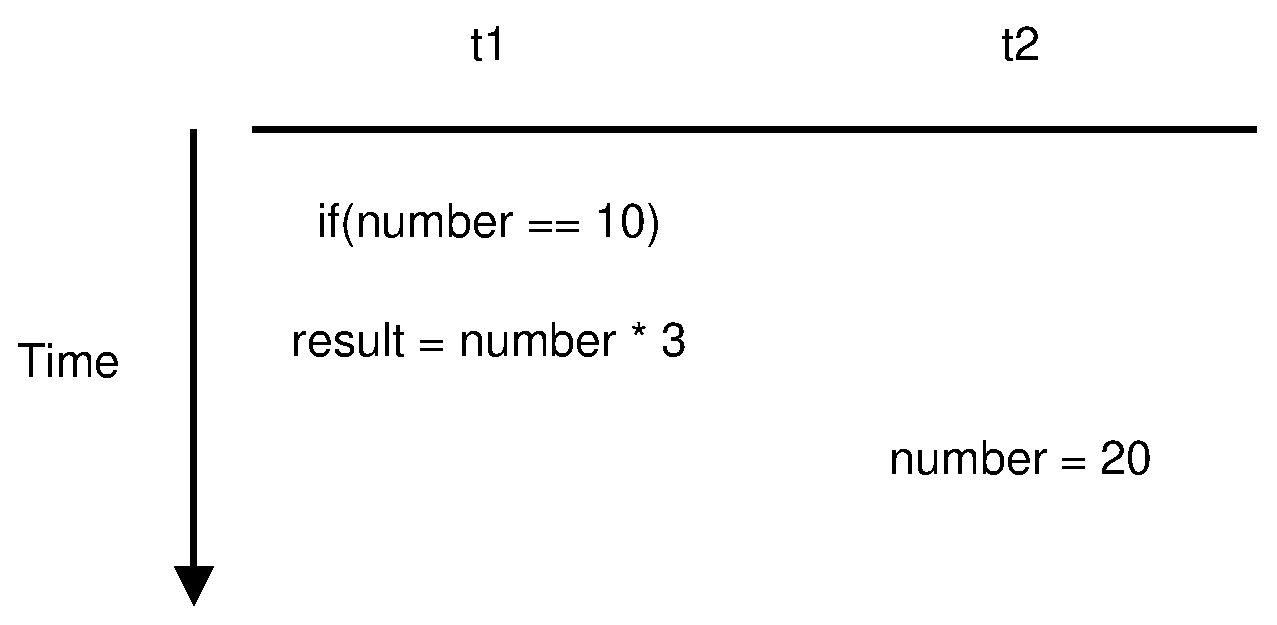
\includegraphics[width=0.65\textwidth]{\rootpath/worksheets/threads_and_locks/figures/race_interleaving1} 
 \caption{First possible interleaving of threads}
\label{fig:race_interleaving1}
\end{figure}

Here it can be seen that \bscode{t1} executes both the evaluation of the if statement and the assignment to result before \bscode{t2} changes value of the number variable. The result is:
\begin{verbatim}
Result is: 30
\end{verbatim}

The second possible result occurs if \bscode{t2} is executed before \bscode{t1}. This interleaving is depicted in \bsref{fig:race_interleaving2}.
\begin{figure}[htbp]
\centering
 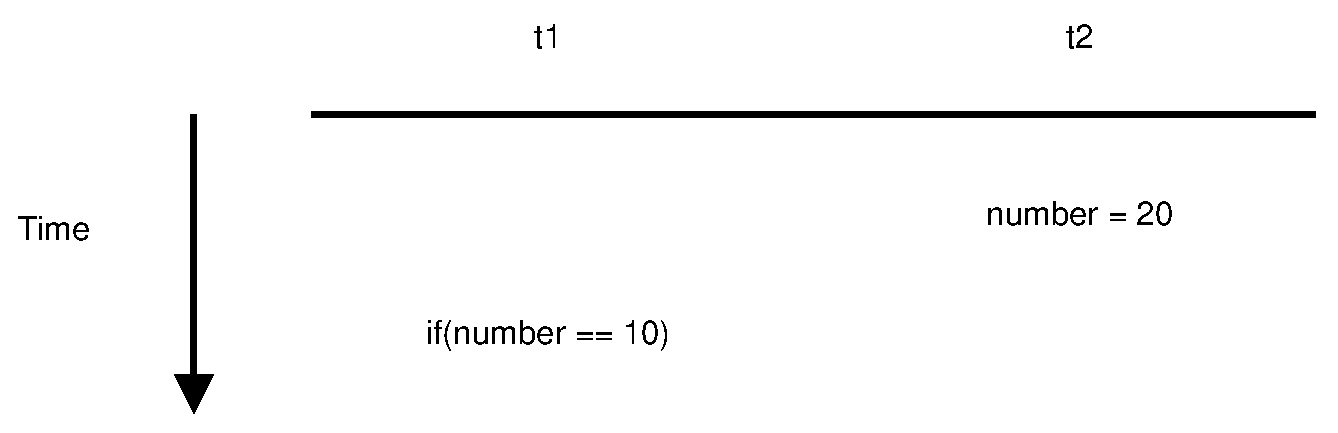
\includegraphics[width=0.65\textwidth]{\rootpath/worksheets/threads_and_locks/figures/race_interleaving2} 
 \caption{Second possible interleaving of threads}
\label{fig:race_interleaving2}
\end{figure}
Here it is shown how \bscode{t2} changes the value of the number variable to 20, before \bscode{t1} has evaluated its precondition. Because of this \bscode{t1} never evaluates the assignment to the result variable and the printed result becomes:
\begin{verbatim}
Result is: 0
\end{verbatim}

The final possible result occurs if \bscode{t1} evaluates the precondition for the if statement on line 7, after which it is paused by the operating system, and \bscode{t2} gets to run instead. \bscode{t2} then changes the value of the number variable which \bscode{t1} just evaluated to be equal to 10. \bscode{t2} then exits and \bscode{t1} is resumed calculating the value assigned to the result variable based on the value of the number value set by \bscode{2}. The result of this is:
\begin{verbatim}
Result is: 60
\end{verbatim}
The third possible interleaving is shown in \bsref{fig:race_interleaving3}. 
\begin{figure}[htbp]
\centering
 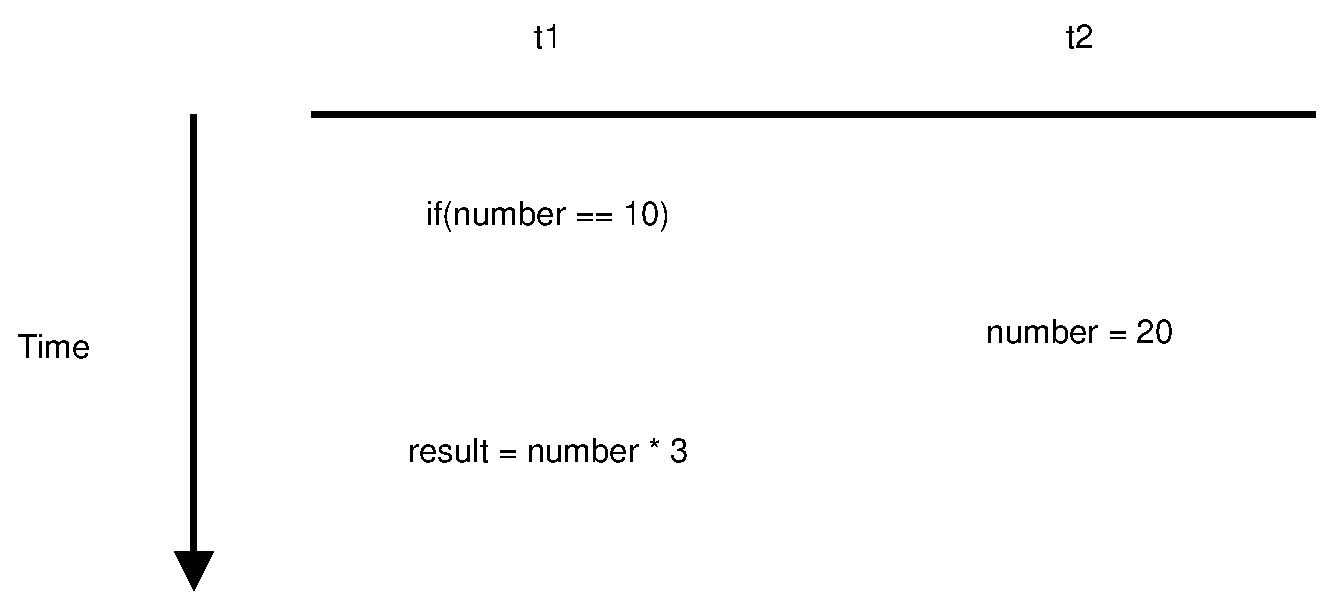
\includegraphics[width=0.65\textwidth]{\rootpath/worksheets/threads_and_locks/figures/race_interleaving3} 
 \caption{Third possible interleaving of threads}
\label{fig:race_interleaving3}
\end{figure}

While the threads in \bsref{fig:race_interleaving1} and \bsref{fig:race_interleaving2} have exclusive access to the number variable, this is not the case in \bsref{fig:race_interleaving3}. The interleaving shown in \bsref{fig:race_interleaving3} does not provide threads with atomic access to the shared number variable, as described in \bsref{sec:synchronization}. As a result, it is not guaranteed that other threads will not access the shared data while a thread is using it, resulting in unintended behaviour by the program.

\subsection{Mutual Exclusion \& Locks}\label{sec:locks_me}
Mutual exclusion is the property of shared memory concurrency which ensures that only a single thread can access a given critical region at a time\cite[p. 117]{tanenbaum2008modern}\cite[p. 962]{bryant2011computer}\cite[p. 6]{herlihy2012art}, a critical region being a thread accessing some memory that is shared with other threads\cite[p. 117]{tanenbaum2008modern}\cite[p. 961]{bryant2011computer}. Mutual exclusion provides atomicity synchronization as dicussed in \bsref{sec:synchronization}. Having only a single thread execute within all critical regions at a time, ensures that the program will behave as if it runs sequentially, even though this might not be the case. Access to critical regions is often restricted by the use of different forms of locks\cite[p. 58]{sutter2005software}. 

Locks are a general class of constructs used for providing mutual exclusion. Locks come in a variety of different forms such a Mutex, Monitor, and Semaphore. Each of these operate in their own way, but the overall goal remains the same. Locks provide mutual exclusion by allowing only a single thread to enter its critical region at a time. When a thread \bscode{t1} attempts to acquire a lock that is already held by another task \bscode{t2},\bscode{t1} blocks, effectively waiting for the \bscode{t2} to exit its critical region and release the lock before proceeding. Locks prevent race conditions but introduce other issues such as: deadlocks, priority inversion, and starvation, which will be presented in \bsref{sec:tl_ci}, and leads to threads spending time blocked instead of executing parts of the program. Furthermore, it is up to the programmer to apply locking to the correct places and in the correct order, which in itself is hard. If he succeeds in using locks as synchronization mechanism, a major caveat is that they are not composable\cite[p. 58]{sutter2005software}. That is, you cannot compose two correct lock-based pieces of code and know the result is still correct. This significantly limits the reuseability of software components.%, and therefore lowers the productivity of the programmer.
\kasper{Maybe move parts of above paragraph to characteristics chapter discussion chapter later}\toby{Eller referer derned til hvis ikke du vil flytte det.}

Consider the example presented in \bsref{lst:mutualexclusion}, which is a modified version of the exampled presented in \bsref{lst:racecondition}. As it can be seen on lines 11-15 and 18-19, the two threads have had their critical regions locked, limiting the access to one thread at a time. If either \bscode{t1} or \bscode{t2} attempts to acquire the lock while the other already holds it, they would block, ensuring mutual exclusion. As a result the interleaving presented in \bsref{fig:race_interleaving3} is no longer possible and the race condition has been removed. 

%\bsref{lst:mutualexclusion} depicts a modified version of the example presented in \bsref{lst:racecondition}. The two threads have had their critical regions locked, limiting the access to one thread at a time. Because of this, the case where \bscode{t1} runs just until its about to compute the result and  \bscode{t2} taking over will no longer occur. \bscode{t2} will now not be able to change the value of number as \bscode{t2} still holds the lock on the critical region, even though it is paused. As a result the output result is: 60, can no longer occur. The output does however still depend on the order in which access to the critical regions is acquired.
\begin{lstlisting}[label=lst:mutualexclusion,
  caption={Mutual exclusion in Java using a lock},
  language=Java,  
  showspaces=false,
  showtabs=false,
  breaklines=true,
  showstringspaces=false,
  breakatwhitespace=true,
  commentstyle=\color{greencomments},
  keywordstyle=\color{bluekeywords},
  stringstyle=\color{redstrings}]  % Start your code-block

	import java.util.concurrent.locks.Lock;
	import java.util.concurrent.locks.ReentrantLock;

	public class MutualExclusion {
    private static int number = 10;
    private static int result = 0;
    private final static Lock lock = new ReentrantLock();

    public static void main(String[] args) throws InterruptedException {
        Thread t1 = new Thread(() -> {
            lock.lock();
            if (number == 10){
                result = number * 3;
            }
            lock.unlock();
        });
        Thread t2 = new Thread(() -> {
            lock.lock();
            number = 20;
            lock.unlock();
        });
        t1.start(); t2.start();
        t1.join(); t2.join();
        System.out.println("Result is: " + result);
    }
	}
\end{lstlisting}

\kasper{Do we want a section on locking constructs such as semaphores and monitores?}\toby{Maybe a short description of the different ones would be nice but i don't think it is something that is absolutely required for the chapter}
%Executor service
%Futres
%Still based on threads

\section{Concurrency Issues}\label{sec:tl_ci}
This section presents an overview of known issues related to \ac{TL} concurrency. Many of the issues arise as a result of locking access to shared memory. Some of the issues are also present in other concurrency models. The overview is used for evaluating the characteristics of the \ac{TL} concurrency model. Furthermore knowing what issues can arise for each of the selected concurrency models, will assist in comparing their complexity.
%Some of the issues are related mainly to shared memory concurrency while others apply to a broader spectrum, including asynchronous message passing.
 
\subsection{Deadlocks}
A deadlock occurs when all threads in a set are waiting on some event, that can only be caused by another thread in the set\cite[p. 435]{tanenbaum2008modern}. Because all the threads are blocked and waiting on one of the other threads, none of them will ever continue and they will block indefinitely.

As an example consider \bsref{fig:deadlockexample}. Here the three threads T1, T2 and T3 are illustrated. The three threads are all waiting on a resource, that has been acquired by one of the other threads, as illustrated by the arrows. Each thread is waiting on a resource held by one of the other threads and is deadlocked. The event the threads are waiting for being the release of the resource.
\begin{figure}[htbp]
\centering
 \includegraphics[width=0.5\textwidth]{\rootpath/worksheets/threads_and_locks/figures/deadlock} 
 \caption{Illustration of a deadlock. All the threads are waiting for the release of a resource held by another thread.}
\label{fig:deadlockexample}
\end{figure}

Deadlocks occur for different reasons in different concurrency models. As described \bsref{fig:deadlockexample} illustrates an example of a deadlock using \ac{TL}. Here the deadlock is caused by threads acquiring a lock on a resource \bscode{R}, where after they attempt to acquire a lock on a resource that is held by another thread, that is directly or indirectly waiting on \bscode{R}. This type of deadlock is called a resource deadlock\cite[p. 435]{tanenbaum2008modern}. 

%Another type of deadlock that can occur in, for example, the Actor concurrency model is called a \emph{communication deadlock}\cite[p. 124]{tanenbaum2008modern}. Instead of deadlocks being caused by locks, a deadlock is here cause by actors waiting on messages. In the context of \bsref{fig:deadlockexample} this would mean that T1, T2 and T3 where actors and the arrows represented an actor waiting on a message from a given actor, so that T1 is waiting on a message from T2. A communication deadlock can occur both over network as well as on a single machine.
%threads and lock = resource aqusision
%async message passing = wating on messages as with resources
\kasper[inline]{Deadlock detection}
\kasper[inline]{Deadlock recovery}

\subsection{Livelocks} A livelock is similar to a deadlock in that no progress is being made. While a deadlocked thread is blocked, a livelocked thread is still executing. The execution does however not result in any progress. A livelock can occur when multiple threads attempts to recover from an error such as a deadlock\cite[p. 457]{tanenbaum2008modern}. Consider two threads \bscode{A} and \bscode{B}. \bscode{A} and \bscode{B} both attempt to write to some common storage, after which they check if the data was written correctly. If that is not the case they attempt the write again. This could lead to another failed attempt and another retry, which could go on indefinitely. \bscode{A} and \bscode{B} are then said to be livelocked.

In this scenario, the livelock could be avoided by having each task wait a random period of time $t < m$, where $m$ is the current maximum wait time, before retrying. Having $m$ grow for each time a task has to retry its operation minimizes the risk of the other tasks interfering with the write as it is more likely that the retry will occur at different times. It is however also of interest to minimize wait time as no progress is made during this period.

\subsection{Priority Inversion}
Priority inversion is the problem of a high priority thread blocking, while waiting for a low priority thread to finish\cite[p. 456]{tanenbaum2008modern}. As an example consider the two threads \bscode{H} and \bscode{L} shown in \bsref{fig:priority_inversion}. \bscode{H} has a high priority while \bscode{L} has a low priority. \bscode{L} starts running, enters its critical region and acquires a lock on some shared resource \bscode{R}. The high priority task \bscode{H} is then started. It attempts to acquire a lock on the resource \bscode{R} in order to enter its critical region. The lock on \bscode{R} is however still held by \bscode{L} and the high priority task \bscode{H} must now wait for the low priority task \bscode{L} to finish.

\begin{figure}[htbp]
\centering
 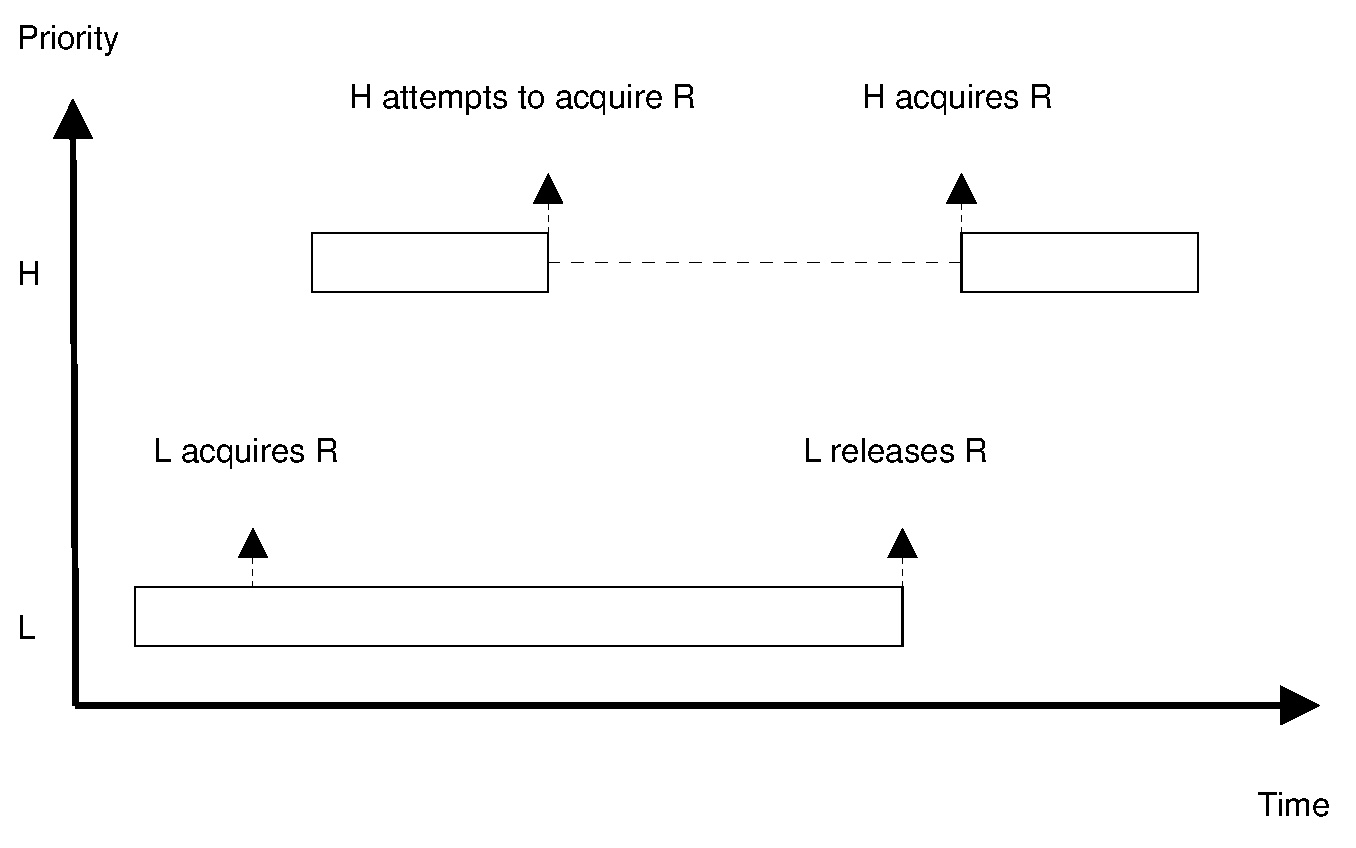
\includegraphics[width=0.95\textwidth]{\rootpath/worksheets/threads_and_locks/figures/pi_graf} 
 \caption{Priority inversion example}
\label{fig:priority_inversion}
\end{figure}
If a thread \bscode{M} with medium priority was introduced that do not need to acquire resource R, the scenario could instead look as depicted in \bsref{fig:priority_inversion_m}. The scenario is similar to the previous but here \bscode{M} starts up after \bscode{L} has acquired the lock on \bscode{R}. Because \bscode{M} is a medium priority task it is scheduled before \bscode{L}. As a result \bscode{H} has to wait on both a low and medium priority task to finish before acquiring the lock on \bscode{R}.

\begin{figure}[htbp]
\centering
 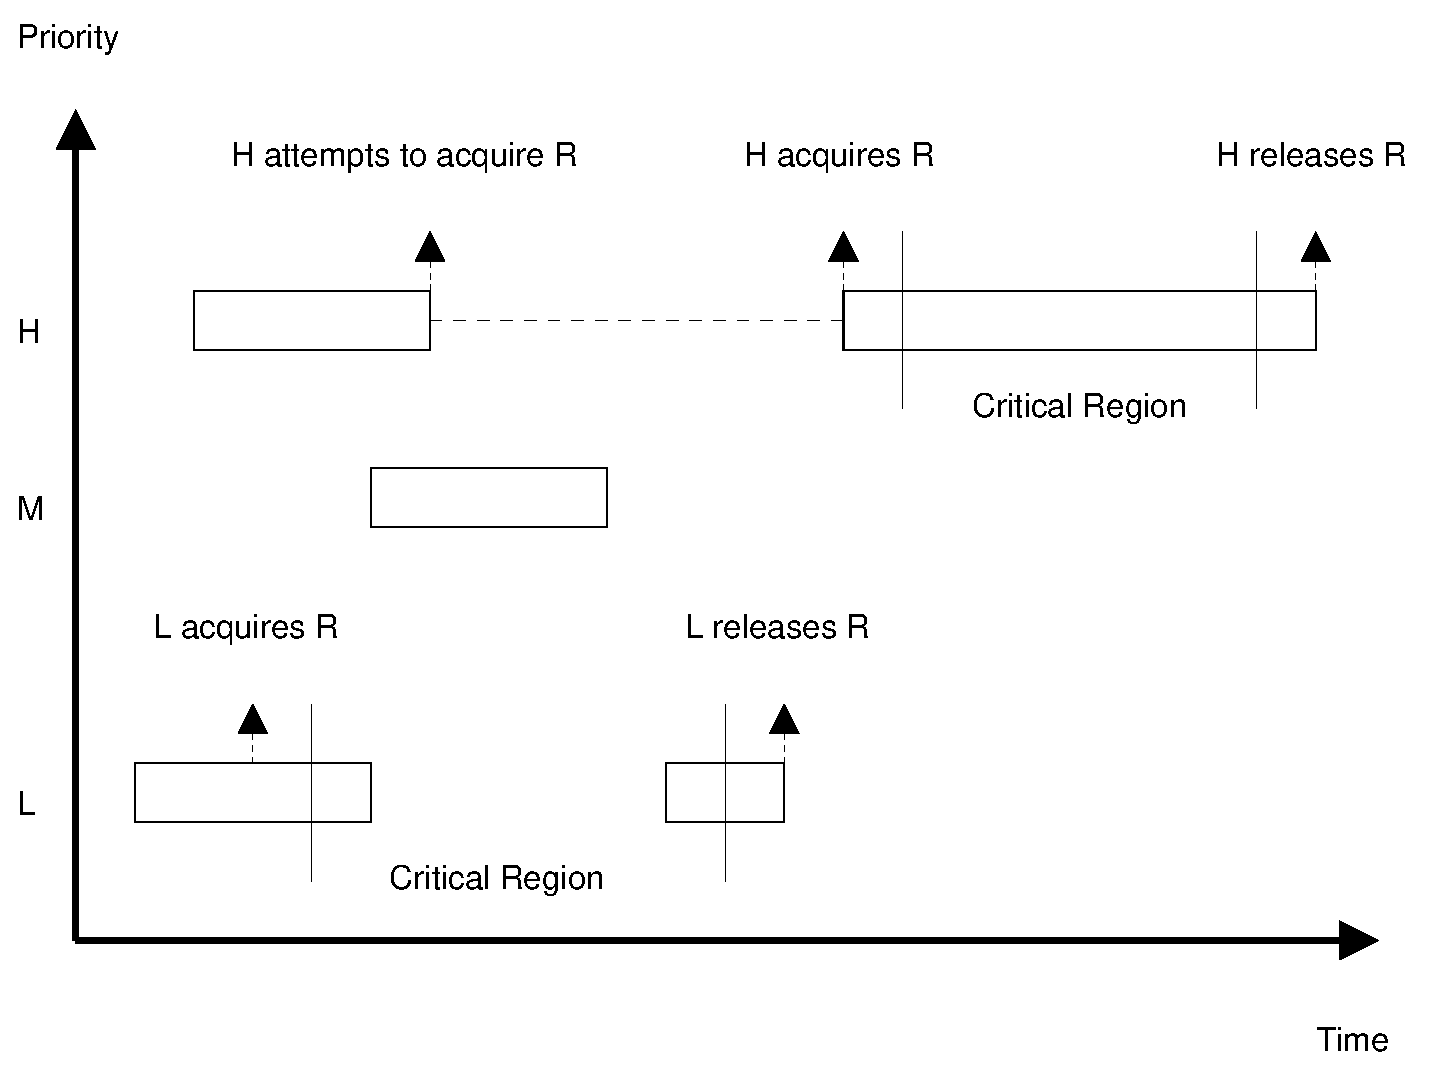
\includegraphics[width=0.95\textwidth]{\rootpath/worksheets/threads_and_locks/figures/pi_graf2} 
 \caption{Priority inversion with medium priority task}
\label{fig:priority_inversion_m}
\end{figure}
%\andreas{Move M so H acquire R before M starts}
\subsection{Starvation}
A thread is said to be starved if, it is denied access to a resource indefinitely\cite[p. 459]{tanenbaum2008modern}. The task can be denied based on many different criteria. For example, priority or the size of the job that it is to perform.

As an example, imagine a scheduler that gives threads access to some resource R based on the priority of the thread. Threads with a high priority gets access to the resource before threads with a low priority. Now imagine a low priority thread \bscode{A} attempts to acquire a lock on some resource \bscode{R}. The lock on \bscode{R} is however currently held by some other task and \bscode{A} is blocked waiting for access to \bscode{R}. While \bscode{A} is blocked, a high priority task \bscode{B} also attempts to acquire the lock on \bscode{R} and is blocked as well. When the lock on \bscode{R} is released it is given to the high priority task \bscode{B} even though \bscode{A} blocked first and \bscode{A} remains blocked. If this scenario keeps repeating and a high priority task keeps getting the lock over \bscode{A}, \bscode{A} is said to be starved.

%The same scenario can without the use of locks for synchronization. Imagine a printing service in a asynchronous message passing system. The printing service accepts, schedules and handles print jobs on behalves of a number of clients. The printing services givers a higher priority to jobs created by some clients than jobs created by others. If a client submitted the low priority job \bscode{A} to the printing service, but the queue of the printing service already contained a number of high priority jobs, \bscode{A} would have to wait until the high priority jobs where finished. If the printing services keeps receiving new high priority jobs at a pace such that the queue allways contains atleast a single high priority job, then \bscode{A} will never be executed and will be starved. The similar scenario could occur if the printing service gave priority to the smallest job. A very large job might starve as smaller jobs keep getting prioritized

Starvation can be avoided using a \ac{LIFO} scheduling strategy\cite[p. 459]{tanenbaum2008modern}.

\section{Discussion}
\label{sec:tl_discussion}
This section contains a discussion of a number of issues related to \ac{TL} concurrency. Why \ac{TL} concurrency is considered to be hard is discussed in \bsref{subsec:tl_lock_hard}, followed by a discussion of the composability of the \ac{TL} concurrency model in \bsref{subsec:tl_composability}.
\subsection{Why locks are hard}\label{subsec:tl_lock_hard}
Concurrency is generally considered to be hard, the same goes for using locks to provide mutual exclusion\cite[p. 56]{sutter2005software}. Several reasons for this exist. One is that in order for locks to work, programmers have to strictly follow a set of conventions. If, for example, the programmer takes locks in the wrong order, it can potentially lead to deadlocks\cite[p. 58]{sutter2005software}. Furthermore the relationship between a lock and the shared data it is protecting is implicit, that is, it is enforced by the programmer. If the programmer misses or leaks a reference to the shared data, mutual exclusion is no longer ensured and race conditions can occur. This is worsened by locking being a global property that requires local handling. That is, data might be shared between many parts of a system, and each part has to locally reason about locking access to the data.

Locks also has the unfortunate problem of not mixing well with some aspects of \ac{OOP}. Encapsulating data within objects that only allow modification to the data via the objects interface, is well known concept from \ac{OOP}, known as encapsulation or information hiding. Ensuring that multiple threads accessing an object does not corrupt its internal structure, can be done by encapsulating locking, along with the data, inside the object. As an example consider the \bscode{Account} class presented in \bsref{lst:account_example}.\toby{Måske forklar hvorfor der bliver brugt en reentrantlock eller brug en almindelig lock til eksemplet? Mener heller ikke vi har forklaret hvad det er før.} The \bscode{Account} class uses an internal lock, which is defined on line 4, to ensure that only a single thread can modify the balance of the account at a time. This solution does however have a number of issues. Firstly, if a programmer was to extend the \bscode{Account} class and provide an overridden version of the credit or debit method, she would have to ensure that mutual exclusion on the balance was maintained. In this simple example such a task could be achieved without too much trouble, assuming that the programmer extending the account class knows about the lock. If however it had been a more complex class, using more sophisticated locking, providing an overridden method might not be a simple task. In any case it is a task with a high potential for programmer error, especially if the programmer does not have access to the source code of the class that is to be extended.

\begin{lstlisting}[float,label=lst:account_example,
  caption={Encapsulated locking},
  language=Java,  
  showspaces=false,
  showtabs=false,
  breaklines=true,
  showstringspaces=false,
  breakatwhitespace=true,
  commentstyle=\color{greencomments},
  keywordstyle=\color{bluekeywords},
  stringstyle=\color{redstrings}]  % Start your code-block

	public class Account {

    private int balance;
    protected final Lock lock = new ReentrantLock();

    public Account(int balance){
       this.balance = balance;
    }

    public void credit(int amount){
        lock.lock();
        balance += amount;
        lock.unlock();
    }

    public void debit(int amount){
        lock.lock();
        balance -= amount;
        lock.unlock();
    }
	}
\end{lstlisting}

Secondly consider the example of transferring funds from one account to another. \bsref{lst:account_example_transfer} shows one way in which this could be achieved. The two accounts \bscode{a1} and \bscode{a2} are created with balances of 500 and 100 respectively. 200 is debited from \bscode{a1} followed by crediting \bscode{a2} with 200 completing the transfer. The problem arises because the encapsulated locking only protects each call to debit and credit but not the transfers as a whole\cite[p. 59]{sutter2005software}. A thread can read the inconsistent state of the accounts in between the debiting of \bscode{a1} and crediting of \bscode{a2}. Additional locking has to be provided  if this is to be avoided.

\begin{lstlisting}[float,label=lst:account_example_transfer,
  caption={Funds transfer between two accounts},
  language=Java,  
  showspaces=false,
  showtabs=false,
  breaklines=true,
  showstringspaces=false,
  breakatwhitespace=true,
  commentstyle=\color{greencomments},
  keywordstyle=\color{bluekeywords},
  stringstyle=\color{redstrings}]  % Start your code-block

    Account a1 = new Account(500);
    Account a2 = new Account(100);
    a1.debit(200);
    a2.credit(200);
\end{lstlisting}

In \cite{lee2006problem} the author argues that introducing threads into a program makes the program nondeterministic, that is, the program can produce different results for each time it is run. This is exactly the effect race conditions, described in \bsref{subsec:race_coditions}, have on a program. The author argue that it becomes the job of the programmer to prune away this nondeterminism in order to produce a deterministic program. Using the \ac{TL} concurrency model this is done using different forms of lock. However such pruning is not an easy task and using the \ac{TL} model introduces a number of other issues such as deadlocks and starvation.

%Some locking constructs, such as Java's syncronized methods, provide object based locking.
%\subsection{\ac{TL} and OOP}

\subsection{Composability}\label{subsec:tl_composability}

As mentioned in \bsref{sec:locks_me}, lock based concurrent implementations are not composable. Creating new software by composing existing implementations, in the form of libraries, is a common practice in software development. As software libraries does not perish on use, it is natural to reuse existing libraries. If such libraries use locks to correctly ensure mutual exclusion, it is not guaranteed that combining these libraries, results in an application free of concurrency related errors.

Deadlocks are the primary reason for locks not composing\cite[p. 58]{sutter2005software}. Event based frameworks call code, that has been defined by programmers using the framework, to signal that some event occurred. If such frameworks use locks to ensure correct synchronization, calling code which the framework itself knows nothing about, while holding locks, can lead to deadlocks.

As an example consider the observer pattern\cite{gamma1994design} in which an object (the observable) is observed by a number of observers. Observers can register and unregister for notifications and the observable notifies any registered observers whenever some event occurs. 

\bsref{lst:observer} shows the implementation of an observable that attempts to use a semaphore in order to ensure thread safety. In this example, the \bscode{Observable} represents the framework, and the \bscode{Observer} represents the client code using the framework. 

The \bscode{ValueStore} class implements the \bscode{Observable} interface, overriding the two methods \bscode{register} and \bscode{unregister} defined on the interface. Besides these two methods the \bscode{ValueStore} class defines the \bscode{setValue} method which allows others to set the stored value as well as triggering a notification to all registered observers. As mentioned the \bscode{ValueStore} class uses a semaphore to ensure mutual exclusion. The semaphore is used to lock access to the \bscode{ValueStore}'s internal value and list of observers. On lines 18-20 and 25-27 the semaphore locks access to the list of observers while while a registration or unregistration is in progress. On lines 8-13 the semaphore locks access to the internal value and list of observers while the value is changed and any registered observers are notified. This prevents changes to the internal value as well as preventing any observers from registering and unregistering, while the value store is notifying existing observers.

\begin{lstlisting}[label=lst:observer,
  caption={Observer pattern with locks},
  language=Java,  
  showspaces=false,
  showtabs=false,
  breaklines=true,
  showstringspaces=false,
  breakatwhitespace=true,
  commentstyle=\color{greencomments},
  keywordstyle=\color{bluekeywords},
  stringstyle=\color{redstrings}]  % Start your code-block

	public class ValueStore implements Observable{

    private int value = 0;
    private List<Observer> observers = new ArrayList<>();
    private Semaphore sem = new Semaphore(1);

    public void setValue(int newValue) throws InterruptedException {
        sem.acquire();
        value = newValue;
        for (Observer o : observers) {
            o.notify(this,value);
        }
        sem.release();
    }

    @Override
    public void register(Observer observer) throws InterruptedException {
        sem.acquire();
        observers.add(observer);
        sem.release();
    }

    @Override
    public void unregister(Observer observer) throws InterruptedException {
        sem.acquire();
        observers.remove(observer);
        sem.release();
    }
	}
	
	public class ValueObserver implements Observer {

    @Override
    public void notify(Observable sender, int value) throws InterruptedException {
        sender.unregister(this);
    }
	}

	public class Main {

    public static void main(String[] args) throws InterruptedException {
        ValueStore observable = new ValueStore();
        observable.register(new ValueObserver());
        observable.setValue(5);
        System.out.println("Done");
    }
	}
\end{lstlisting}

The \bscode{ValueObserver} class implements the observer interface and overrides its notify method. The notify method simply unregisters from the observable supplying the notification.

The \bscode{Main} class and its \bscode{main} method defines the behaviour of the program. On line 42 a \bscode{ValueStore} is created followed by the registration of a \bscode{ValueObserver}, setting the value of the \bscode{ValueStore} to 5 and printing \bscode{"Done"} to the console. The printing will however never occur as the program deadlocks before it can happen. The deadlock occurs because the \bscode{ValueObserver} attempts to unregister from the \bscode{ValueStore} while the \bscode{ValueStore} hold the lock. As part of setting the value on line 44 the \bscode{ValueStore} acquires the lock, sets the value and proceeds to notify all observes while still holding the lock, as seen on lines 8-13. Notifying an observer entail calling its \bscode{notify} method, which in the case of the \bscode{ValueObserver} means the \bscode{ValueObserver} unregistering from the observable. As the \bscode{unregister} method attempts to acquire the lock currently held by the \bscode{ValueStore} within the \bscode{setValue} method, a deadlock is created resulting in the \bscode{"Done"} string never being printed.

In order to remove the deadlock one could move the notification of observers in the \bscode{setValue} method outside of the locked section. This would however mean that access to the list of observers would not be thread safe as nothing prevents the registration and unregistration of observers while the \bscode{setValue} method iterates over it. One way to solve this, would be to produce a shallow copy of the observer list within the locked section and iterate over the copy outside the locked section. This eliminates the call to outside defined code while holding locks. This idea is exemplified in the update version of the \bscode{setValue} method depicted in \bsref{lst:observer_updated}.

\begin{lstlisting}[float,label=lst:observer_updated,
  caption={Observer pattern with locks},
  language=Java,  
  showspaces=false,
  showtabs=false,
  breaklines=true,
  showstringspaces=false,
  breakatwhitespace=true,
  commentstyle=\color{greencomments},
  keywordstyle=\color{bluekeywords},
  stringstyle=\color{redstrings}]  % Start your code-block

    public void setValue(int newValue) throws InterruptedException {
        List<Observer> shallowCopy;
        sem.acquire();
        value = newValue;
        shallowCopy = new ArrayList<>(observers);
        sem.release();

        for (Observer o : shallowCopy) {
            o.notify(this,newValue);
        }
    }
\end{lstlisting}

%As an example imagine if that the programmer defined code takes the attempts to acquire the same lock that the framework currently holds.  Because the framework holds the locks 

\section{\acl{TL} Characteristics}
\label{sec:tl_characteristics}
This section presents how the \ac{TL} concurrency model relates to the selected characteristics presented in \bsref{chap:char}.

\subsection{Implicit or Explicit Concurrency}
As described in \bsref{subsec:threads_shared_memory}, the \ac{TL} concurrency model specifies concurrency and synchronization by starting threads and accessing shared memory. Correctness is assured by locking access to critical regions. All of these operations are explicitly stated by the programmer. As such we say that the \ac{TL} concurrency model explicitly states concurrency. The placement is visualized in \bsref{fig:char_implicit_explicit}.

\begin{figure}[htbp]
\centering
 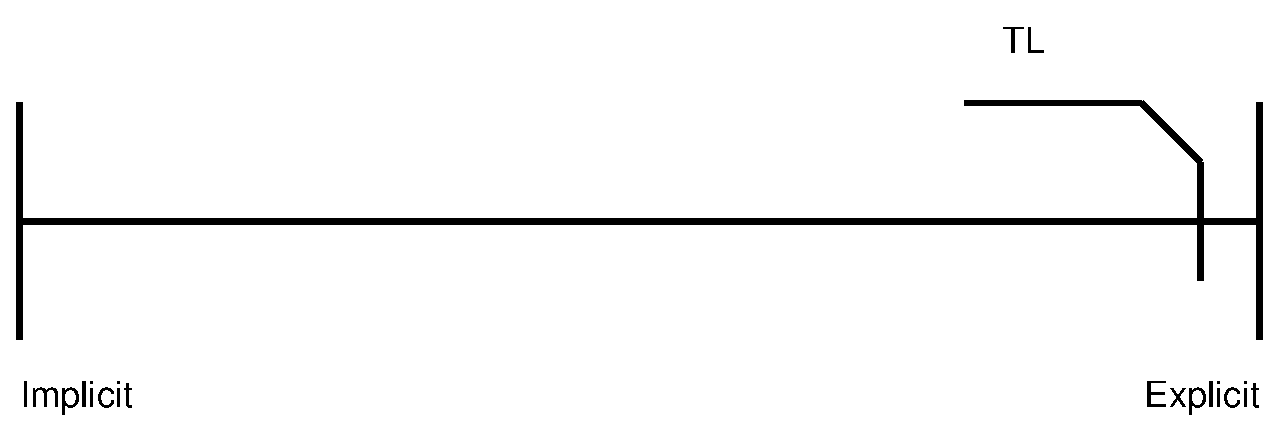
\includegraphics[width=0.9\textwidth]{\rootpath/worksheets/threads_and_locks/figures/tl_char_implicit_explicit} 
 \caption{\ac{TL} on the implicit - explicit concurrency spectrum}
\label{fig:char_implicit_explicit}
\end{figure}

\subsection{Fault Restrictive or Expressive Model}
\ac{TL} forces very little upon the programmer. The programmer is left alone to ensure correct execution using locks as well as deciding on a fitting lock granularity. The programmer is given a lot of freedom in expressing concurrency at the cost of having to ensure correct execution herself. Based on these observations we say that \ac{TL} is an expressive concurrency model as shown in \bsref{fig:char_fault_expressive}.

\begin{figure}[htbp]
\centering
 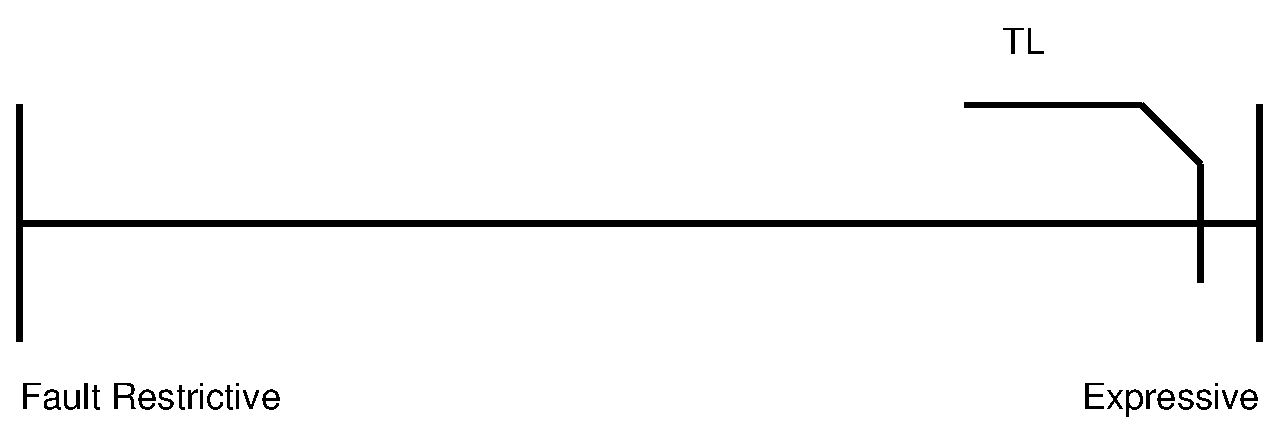
\includegraphics[width=0.9\textwidth]{\rootpath/worksheets/threads_and_locks/figures/tl_char_fault_expressive} 
 \caption{\ac{TL} on the fault restrictive - expressive spectrum}
\label{fig:char_fault_expressive}
\end{figure}

\subsection{Pessimistic or Optimistic Model}
As described in \bsref{sec:locks_me}, the \ac{TL} concurrency model uses locks to ensure mutual exclusion in order to eliminate race conditions. That is, the \ac{TL} concurrency model uses locks to eliminate errors. \ac{TL} assumes that errors will occur and attempts to prevent them. Furthermore, \ac{TL} provides no options for recovery in case of errors. Based on these observations we say that \ac{TL} is a pessimistic model as shown in \bsref{fig:char_pes_opti}.

\begin{figure}[htbp]
\centering
 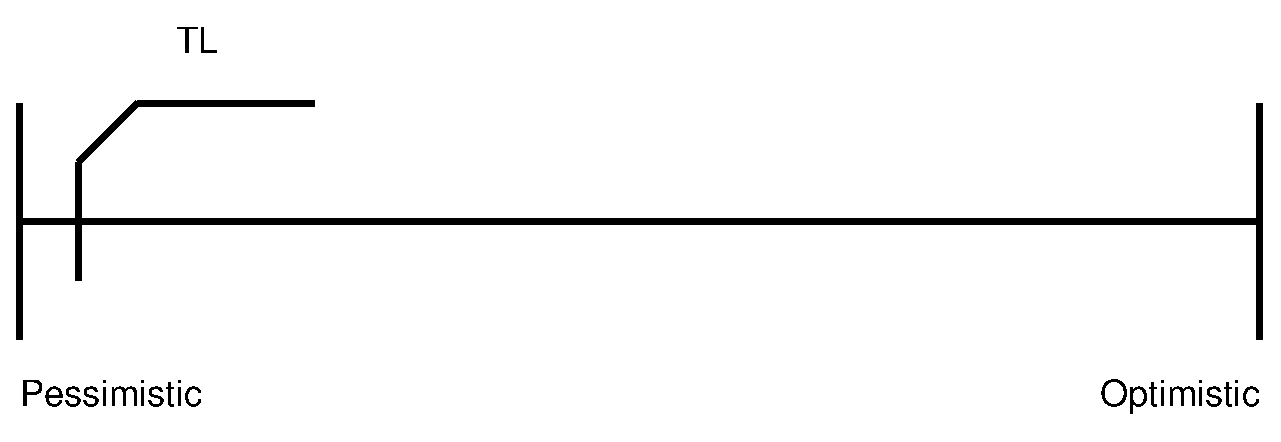
\includegraphics[width=0.9\textwidth]{\rootpath/worksheets/threads_and_locks/figures/tl_char_pessimistic_optemistic} 
 \caption{\ac{TL} on the pessimistic - optimistic spectrum}
\label{fig:char_pes_opti}
\end{figure}

\subsection{Readability \& Writability}\label{subsec:tl_charac_read_and_write}
As mentioned in \bsref{sec:readability} and \bsref{sec:writablity}, the evaluation of readability and writablity will be based upon the evaluation of the sub characteristics, on which they are based. As two of these, simplicity and orthogonality, are common for both readability and writability, an evaluation of these is presented first. After this, an evaluation of the readability properties of the \ac{TL} concurrency model is presented, followed by the evaluation of \ac{TL} concurrency models level of abstraction and expressivity. Finally an evaluation of the writability of the \ac{TL} concurrency model is presented.

%that of simplicity and orthogonality as well as a number of other considerations. Simplicity and orthogonality is described in the following sections followed by a final evaluation of readability.
\subsubsection{Low or High Simplicity}\label{subsec:tl_simplicity_read}
As described in \bsref{subsec:tl_lock_hard} and \bsref{subsec:tl_composability} the \ac{TL} concurrency model has a number of issues which contribute negatively to its simplicity. When taking multiple locks, taking them in incorrect order might result in a deadlock. Locking is however, as described in \bsref{subsec:tl_lock_hard}, a global property and the correct order might not be directly discernible by the reader, from within the local context. As such it is no simple task for the reader to reason about the order of locking.

\bsref{subsec:tl_composability} describes how the \ac{TL} model is not composable. Implementing the observer pattern in a thread safe manner was shown to entail a number of issues. The potential for concurrency related programmer errors in similar implementations is high and identifying these errors can potentially be a non trivial task.

In \cite{lee2006problem} the author describes development of the Ptolemy project\cite{lee1999overview}, which involved a significant aspect of concurrency. During the development phase of this project, the software engineering approaches of design reviews, code reviews, nightly builds, regression tests, and automated code coverage metrics where employed in order to produce a bug free program\cite[p. 8]{lee2006problem}. Even though the team achieved 100\% code coverage and all code was reviewed by experts, the system still deadlocked after having been in production for four years, indicating that employing good software engineering principles, might not be enough to catch all concurrency related errors, even among experts.

Based on the issues mentioned here, as well as the sheer number of concurrency related issue that can arise when using the \ac{TL} concurrency model, we say that the \ac{TL} model has low simplicity. Its placements on the simplicity spectrum is depicted in \bsref{fig:char_read_simplicity}.

\begin{figure}[htbp]
\centering
 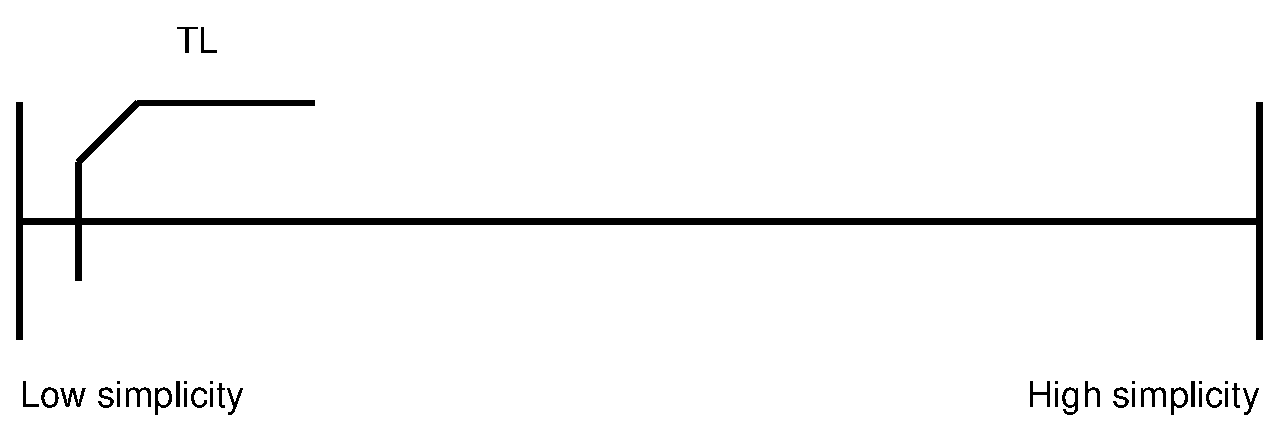
\includegraphics[width=0.9\textwidth]{\rootpath/worksheets/threads_and_locks/figures/tl_char_read_simplicity} 
 \caption{\ac{TL} on the low - high simplicity spectrum}
\label{fig:char_read_simplicity}
\end{figure}

\subsubsection{Low or High Orthogonality}\label{sec:tl_orthogonality}
The \ac{TL} concurrency model consists of only a few constructs. Threads are started in order to introduce concurrency and synchronization is achieved using some form of locking. These basic constructs can be combined in a large number of ways, in order to produce concurrent programs. As such the \ac{TL} concurrency model seems to be orthogonal as it consists of a small number of constructs, which can be combined in a large number of ways. Each of the constructs does however have its own distinct purpose, which means that only certain combinations of the constructs are useful. In fact some erroneous combinations can lead to serious issues such as deadlocks. We say that the \ac{TL} concurrency model is towards the high orthogonality end of the low - high orthogonal spectrum. This was chosen based on the number of constructs and combinations of these. The fact that some combinations can lead to program errors which are hard to detect has however kept the \ac{TL} concurrency model from being considered truly orthogonal. The placement of the \ac{TL} concurrency model on the low - high orthogonal spectrum is depicted in \bsref{fig:char_tl_orthogonality}.

\begin{figure}[htbp]
\centering
 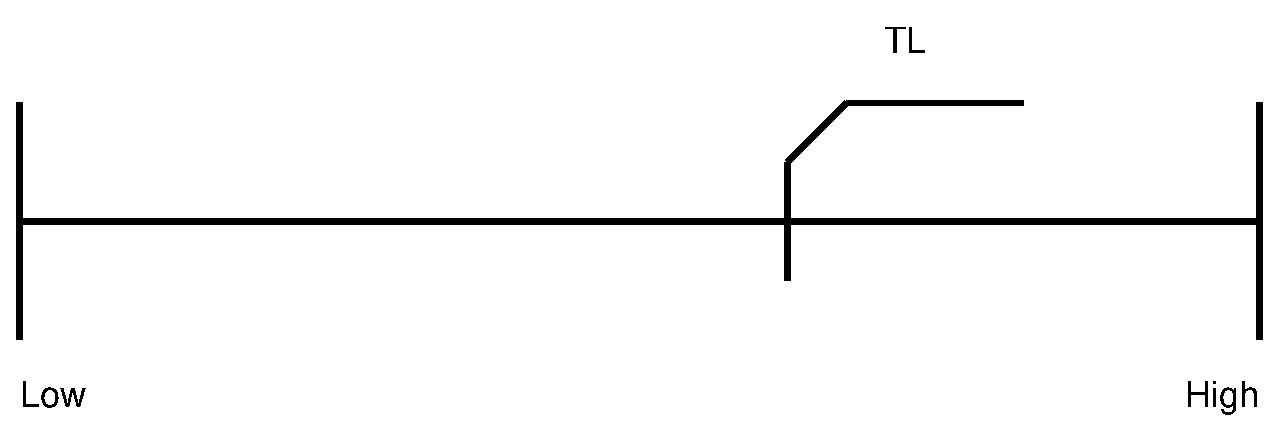
\includegraphics[width=0.9\textwidth]{\rootpath/worksheets/threads_and_locks/figures/tl_char_orthogonality} 
 \caption{\ac{TL} on the low - high orthogonality spectrum}
\label{fig:char_tl_orthogonality}
\end{figure}

\subsubsection{Low or High Readability}
\label{subsec:tl_char_readability}
As described in \bsref{subsec:tl_simplicity_read} the simplicity of the \ac{TL} model as residing in the low end of the low - high simplicity spectrum. In \bsref{sec:tl_orthogonality} say that the orthogonality resides slightly towards the high end of the low - high orthogonality spectrum. These results directly influence the readability of the \ac{TL} concurrency model.

\ac{TL} based concurrency implementations can be very fragmented. Shared memory can be accessed from different parts of the program and requires locking in each of these places. When a programmer reads the code present at one of these places, she can choose to focus only on understanding this part of the code, reducing the scope of what she has to reason about. Doing so will however only allow the programmer to understand this segment of the code, but not reason about its correctness as this depends on the code present at every place where the shared memory is accessed. Reasoning about the correctness of a \ac{TL} based implementation, requires knowledge of all these places and is generally considered to be a non trivial task.

Considering this as well as the evaluation of simplicity and orthogonality we say that the \ac{TL} concurrency model is on the low end of the low - high readability spectrum. The main reason for this assessment being the low simplicity of the model, which makes it hard to reason about the correctness of a implementation. Gathering the intent of a code segment locking access to some shared memory is relatively straight forward, but reasoning about the correctness of the code, in the context of the entire systems, is much harder. The number of issues that the programmer has to reason about when determining correctness further exacerbates the issue. The placement of the \ac{TL} concurrency model on the low - high readability spectrum is depicted in \bsref{fig:char_tl_readability}.

\begin{figure}[htbp]
\centering
 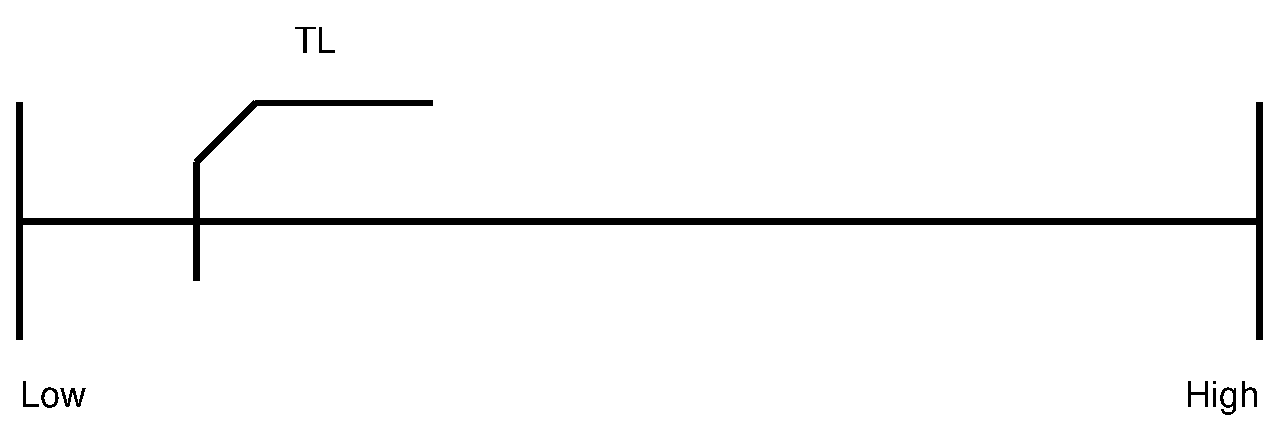
\includegraphics[width=0.9\textwidth]{\rootpath/worksheets/threads_and_locks/figures/tl_char_readability} 
 \caption{\ac{TL} on the low - high readability spectrum}
\label{fig:char_tl_readability}
\end{figure}

\subsubsection{Low or High Level of abstraction}\label{sec:tl_level_of_abstraction}
The \ac{TL} concurrency model is tightly coupled with the underlying hardware architecture. Threads are part of the process model used in the \ac{OS} and the \ac{TL} concurrency model directly uses threads in order to introduce concurrency. Synchronization happens via shared memory which is also part of the process model. The locking is done via supporting hardware instructions such as Test-and-set or Compare-and-swap\cite[p. 1990]{scott2011sync}. Many languages now include more high level abstractions, such as Java's ExecutorService\footnote{\url{http://docs.oracle.com/javase/7/docs/api/java/util/concurrent/ExecutorService.html}}, which hide the underlying threads from the programmer. However, generally such abstractions still use threads underneath. Because the abstractions which the \ac{TL} concurrency model offers is so tightly coupled with the hardware and \ac{OS}, we say that the \ac{TL} concurrency model has a low level of abstraction. The placement of the \ac{TL} concurrency model on the low - high level of abstraction spectrum is depicted in \bsref{fig:char_tl_readability}.

\begin{figure}[htbp]
\centering
 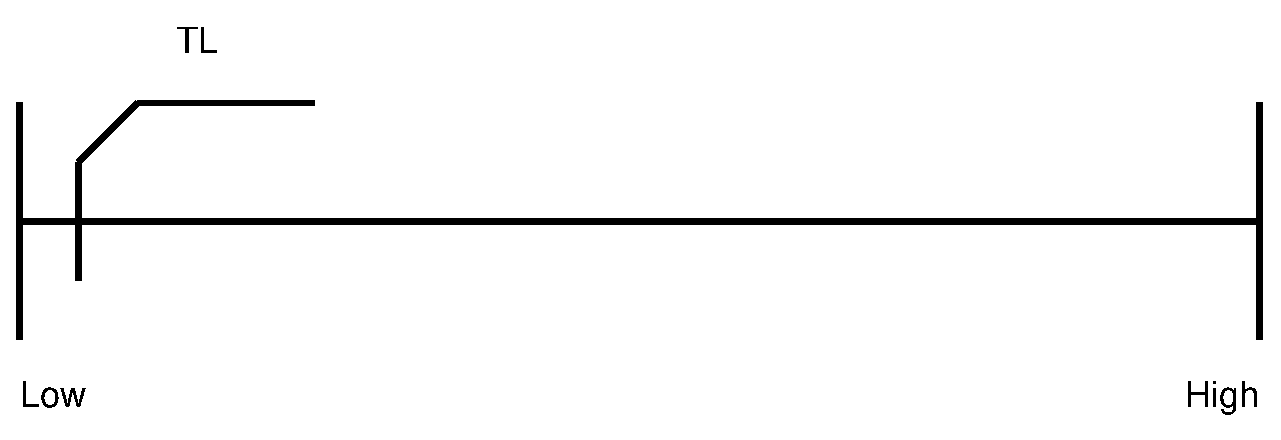
\includegraphics[width=0.9\textwidth]{\rootpath/worksheets/threads_and_locks/figures/tl_char_level_of_abstraction} 
 \caption{\ac{TL} on the low - high level of abstraction spectrum}
\label{fig:char_tl_level_of_abstraction}
\end{figure}

\subsubsection{Low or High Expressivity}\label{sec:tl_expressivity}
The expressivity of the \ac{TL} concurrency model is tightly coupled with its level of abstraction. As the constructs that \ac{TL} offers are so close to the hardware primitives, the expressivity of the \ac{TL} concurrency model suffers.

Using the \ac{TL} concurrency model, concurrency is expressed by starting threads and locking access to critical regions. Starting a thread to introduce concurrency is a low level operation, directly related to the process model discussed in \bsref{sec:processes_threads}.

As with starting threads, locking is a low level construct. As discussed in \bsref{sec:locks_me} locking introduces a number of issues which are left up to the programmer to handle. Having to consider these issues limits the expressivity of the model.

Based on these considerations, we say that the \ac{TL} concurrency model has low expressivity. The placement of the \ac{TL} concurrency model on the low - high expressivity spectrum is depicted in \bsref{fig:char_tl_expressivity}.

\begin{figure}[htbp]
\centering
 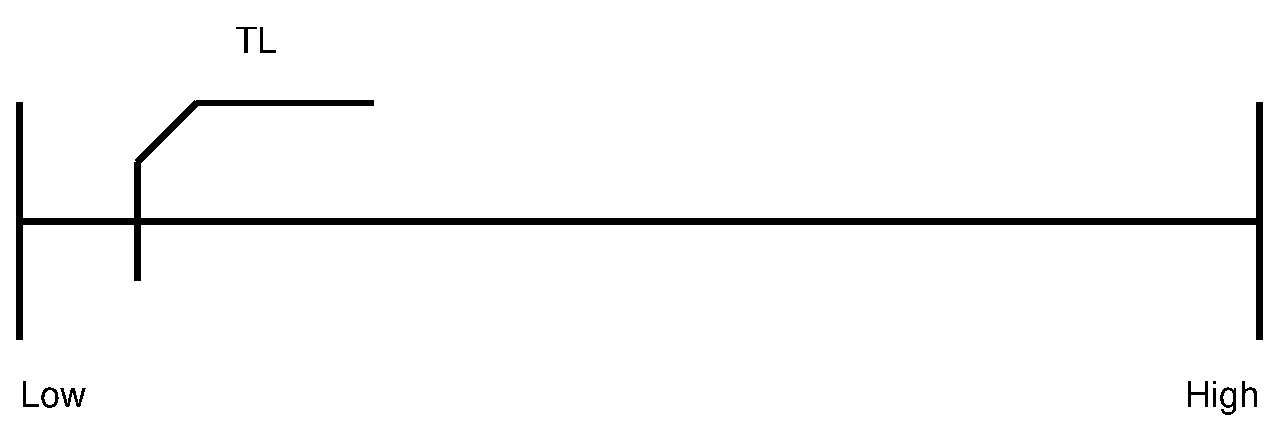
\includegraphics[width=0.9\textwidth]{\rootpath/worksheets/threads_and_locks/figures/tl_char_expressivity} 
 \caption{\ac{TL} on the low - high expressivity spectrum}
\label{fig:char_tl_expressivity}
\end{figure}

\subsubsection{Low or High Writability}
Writing correct \ac{TL} based concurrent implementations is generally considered to be hard\cite[p. 56]{sutter2005software}. As discussed in \bsref{sec:tl_level_of_abstraction}, the \ac{TL} concurrency model has a low level of abstraction where the programmer has to deal with a number of low level details. As a result the programmer is in control of these details but is also forced to manage them limiting the writability of the model.

As discussed in \bsref{sec:tl_expressivity} the \ac{TL} concurrency model has low expressivity, which in turn limits the writablity of the model. If it is cumbersome to correctly express concurrency, writing a concurrent implementation naturally becomes more cumbersome.

The orthogonality of the \ac{TL} concurrency model contributes positively to its writability. Having only a few basic constructs makes it easier for the programmer to learn, recall and use them. As combining these constructs correctly is a non trivial task, the positive effect of the \ac{TL} concurrency models orthogonality properties is limited, resulting in only limited impact on the models writability.

As discussed in \bsref{subsec:tl_simplicity_read}, providing mutual exclusion by locking access to critical regions is a cumbersome task, which is left up to the programmer. While starting threads to introduce concurrency is a relatively simple task, locking requires the programmer to reason about every part of the program in which synchronization is to be made. If the programmer misses just one of these parts, it can introduce race conditions. Furthermore if the programmer makes mistakes while implementing the required locking, it can lead to serious errors such as deadlocks.

In \bsref{sec:tl_ci} a number of concurrency related issues which can arise in the \ac{TL} concurrency model is discussed. Programmers using the \ac{TL} concurrency model have to considerer these issues, which contributes negatively to the models writability. The programmer is forced to think about how these issues can be avoided, which in turn limits the mental effort the programmer can put into producing a concise implementation. Furthermore, having factor these issues in, decreases the productivity of the programmer.

Based on these observations, as well as the evaluation of simplicity and orthogonality, we say that the \ac{TL} concurrency model has low writability. The placement of the \ac{TL} concurrency model on the low - high writability spectrum is depicted in \bsref{fig:char_tl_writability}.

\begin{figure}[htbp]
\centering
 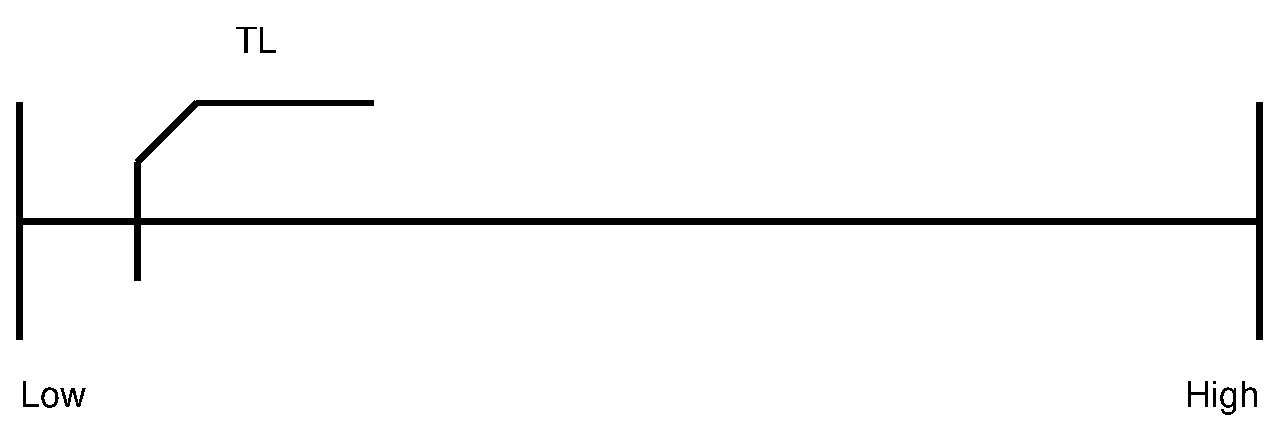
\includegraphics[width=0.9\textwidth]{\rootpath/worksheets/threads_and_locks/figures/tl_char_writability} 
 \caption{\ac{TL} on the low - high writability spectrum}
\label{fig:char_tl_writability}
\end{figure}

\worksheetend
